 %************************************************
\chapter{Understanding Pathology Decoding With
Invertible Networks}\label{understanding-pathology}
%**************************************
\vspace{2em}
\begin{startbox}{EEG-InvNet and EEG-CosNet can reveal learned features for EEG pathology decoding}
\item EEG-InvNet can reach 85.5% accuracy, competitive with regular ConvNets
\item Visualizations show networks learn well-known features like temporal slowing or occipital alpha
\item Visualizations also reveal surprising learned features in the very low frequencies up to 0.5 Hz
\end{startbox}


    After our initial work on pathology decoding, we wanted to gain a deeper
understanding of the features deep networks learn to distinguish healthy
from pathological recordings. For that, we used invertible networks as
generative classifiers since they offer more ways to visualize their
learned prediction function in input space. Our EEG-InvNet reached
competitive accuracies on the pathology decoding task. We visualize
prototypes of the two classes as well as individual electrode signals
predictive of a certain class independent of the signals at other
electrodes. These visualizations revealed both well-known features like
temporal slowing or occipital alpha as well as surprising patterns in
the very low frequencies (\textless= 0.5 Hz). To gain an even better
understanding, we distilled the invertible network's knowledge into a
very small network called EEG-CosNet that is interpretable by design.
These visualizations showed regular patterns in the alpha and beta range
associated with healthy recordings and a diverse set of more irregular
waveforms associated with pathology. For the very low frequencies,
visualizations revealed a frontal component predicting the healthy class
and other components with spatial topographies including the temporal
areas predicting the pathological class.

All work presented in this chapter is novel unpublished work performed
by me in the context of this thesis.

\section{Dataset, Training Details and Decoding
Performance}\label{dataset-training-details-and-decoding-performance}

\begin{table}[h!tb]
    \myfloatalign
    \begin{tabularx}{\textwidth}{p{0.15\textwidth}p{0.15\textwidth}p{0.15\textwidth}p{0.15\textwidth}p{0.15\textwidth}}
    \toprule
        \tableheadlinewithwidth{0.15\textwidth}{Deep} &
        \tableheadlinewithwidth{0.15\textwidth}{Shallow} &
        \tableheadlinewithwidth{0.15\textwidth}{TCN} &
        \tableheadlinewithwidth{0.15\textwidth}{EEGNet} &
        \tableheadlinewithwidth{0.15\textwidth}{EEG-InvNet} \\ 
        \midrule
84.6 & 84.1 & 86.2 & 83.4 & 85.5 \\
        \bottomrule
    \end{tabularx}
    \caption[Accuracy of EEG-InvNet on pathology decoding]{
    \textbf{Accuracy of EEG-InvNet on pathology decoding.} Accuracies of regular ConvNets taken from \citet{gemein2020machine}.
    }  \label{table-tuh-invertible-accuracy}
\end{table}


    We apply our EEG-InvNet to pathology decoding on the same TUH dataset as
in \Cref{pathology}. We use only 2 minutes of each recording at
64 Hz, and input 2 seconds as one example to the invertible network.
This reduced dataset allows fast experimentation while still yielding
good decoding performance. We used AdamW
\citep{DBLP:conf/iclr/LoshchilovH19} as our optimizer and
cosine annealing with restarts
\citep{DBLP:conf/iclr/LoshchilovH17} every 25 epochs as our
learning rate schedule. We emphasize these details were not heavily
optimized for maximum decoding performance, but rather chosen to obtain
a robustly performing model worth investigating more deeply. Results in
\Cref{table-tuh-invertible-accuracy} show that our
EEG-InvNet compares similar than regular ConvNets, even better than some
ConvNets, therefore motivating a deeper investigation into its learned
features.

\section{Class Prototypes}\label{class-prototypes}

\begin{figure}[h!tb]
    \myfloatalign
    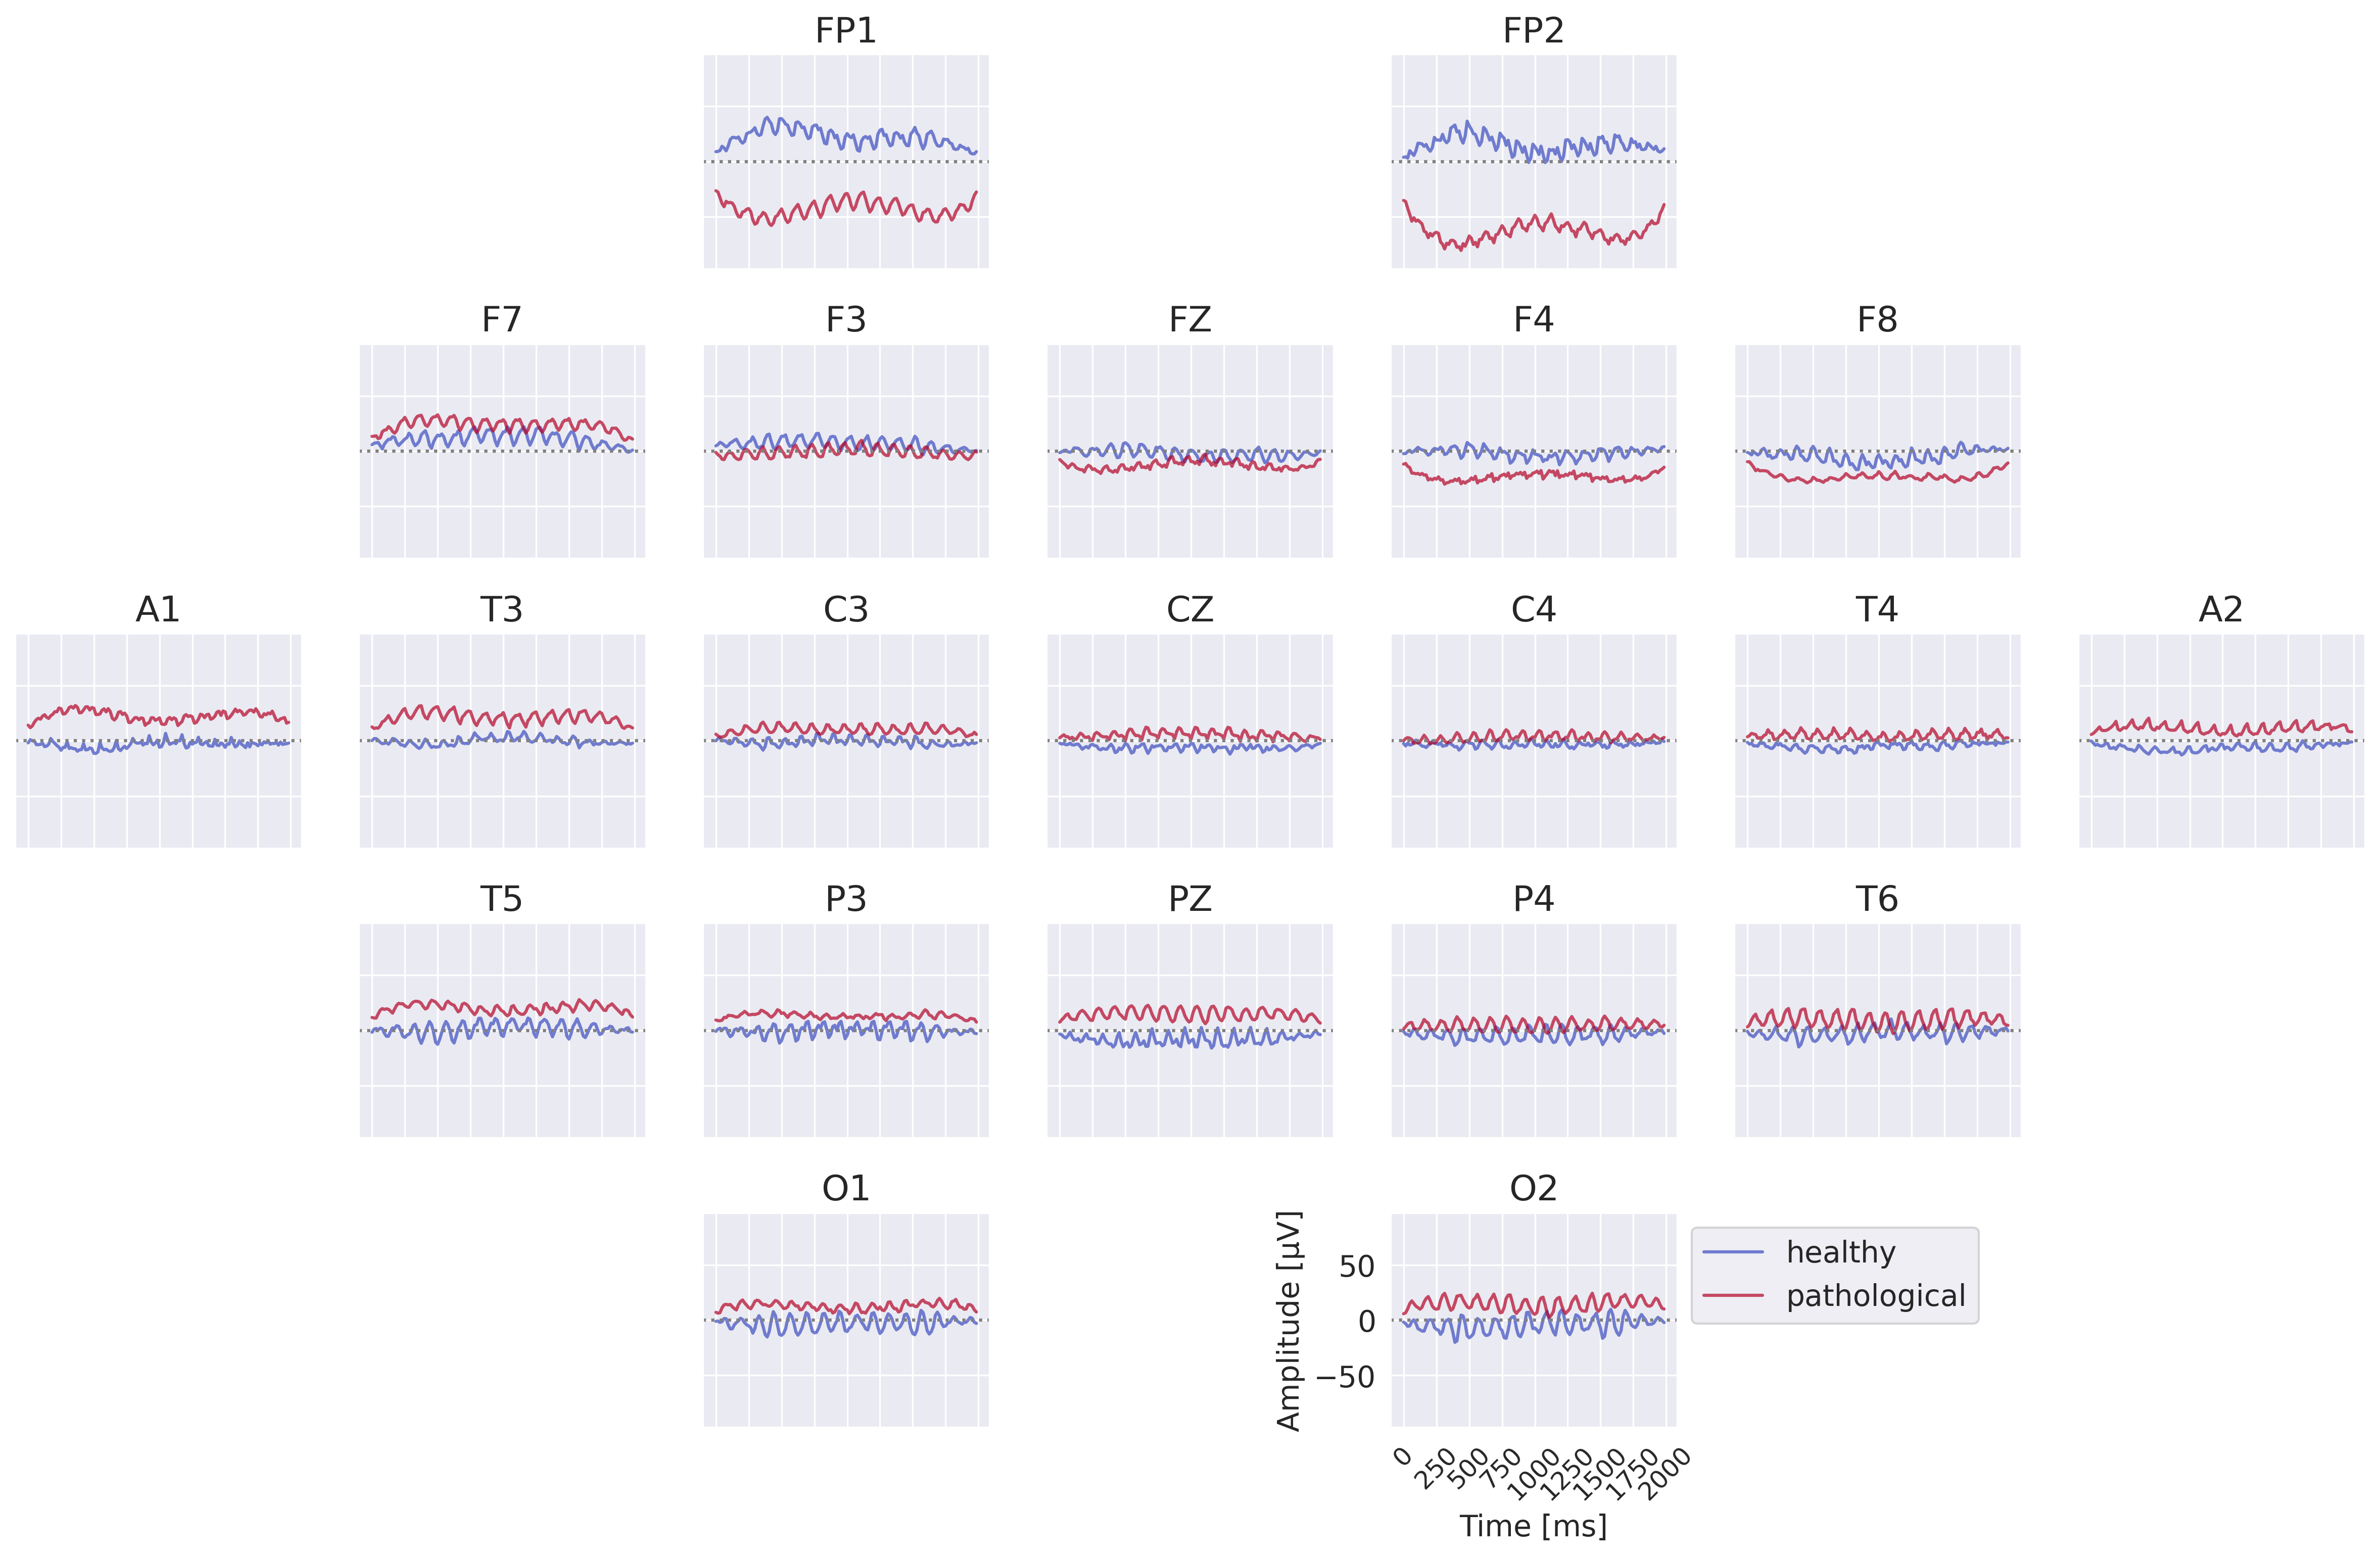
\includegraphics[width=.9\linewidth]{images/net-disc-prototypes.png}
    \caption[Learned class prototypes from EEG-InvNet]{
\textbf{Learned class prototypes from EEG-InvNet.} Obtained by inverting
learned means of class-conditional gaussian distributions from latent
space to input space through the invertible network trained for
pathology decoding.
}
\label{disc-invnet-prototypes}
\end{figure}



    Class prototypes reveal known oscillatory features and surprisingly hint
at the use of very-low-frequency information by the invertible network.
We inverted the learned latent means of the healthy and the pathological
class distributions back to the input space to visualize the most likely
healthy and most likely pathological examples under the learned
distribution, see also \Cref{methods-class-prototypes}.
Visualizations in \Cref{disc-invnet-prototypes} show
differences in the alpha rhythm like a stronger alpha rhythm at O1 in
the healthy example. We also see further differences with a variety of
different oscillatory patterns present for both classes. Surprisingly,
there are also differences in the very low frequencies like
substantially different mean values for FP1 and FP2 for the two class
prototypes, which we will further investigate later. One challenge of
this visualization is that one has to look at each prototype as one
complete example and cannot interpret signals at individiual electrodes
independently. This is what we tackle in our next visualization.

\section{Per-Electrode Prototypes}\label{per-channel-prototypes}

\begin{figure}[h!tb]
    \myfloatalign
    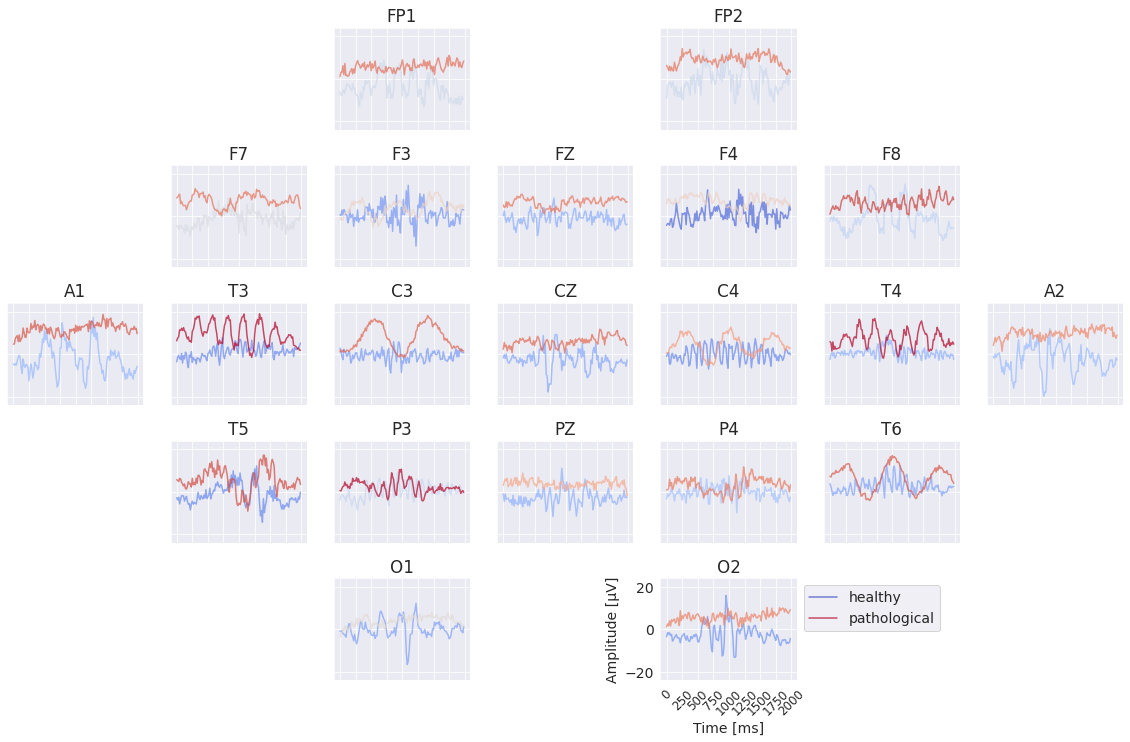
\includegraphics[width=.9\linewidth]{images/marginal-chan-6.png}
    \caption[Learned per-electrode prototypes from EEG-InvNet]{
\textbf{Learned per-electrode prototypes from EEG-InvNet.} Each electrodes'
input is optimized independently to increase the invertible networks
prediction for the respective class. During that optimization, signals
for the other non-optimized electrodes are sampled from the training data.
Color indicates average softmax prediction over 10000 samples for the
other electrodes. Very prominent slowing patterns appear for the
pathological class at multiple electrodes.
}
\label{marginal-chan}
\end{figure}


    The per-channel prototypes reveal interesting learned features for the
two classes (see \Cref{marginal-chan}). The pathological
prototypes show strong low-frequency activity, for example at T3 and T4,
consistent with slowing as a biomarker for pathology. The healthy signal
shows alpha activity, for example at C4 and T6. Besides these patterns,
a lot of other interesting patterns may be interesting to further
investigate. One of them, the differences in the very low frequencies
will be further explored below. Note that it was not possible to
synthesize a signal that is clearly indicative of one class independent
of the other electrodes for all electrodes. This is to be expected if
the EEG-InvNet uses a feature inherently impossible to recreate within a
single electrode like the degree of synchrony between signals at
different electrodes.

\section{EEG-CosNet Visualizations}\label{eeg-cosnet-visualizations}


\begin{table}[h!tb]
    \myfloatalign
    \begin{tabularx}{\textwidth}{p{0.2\textwidth}p{0.3\textwidth}p{0.3\textwidth}}
    \toprule
        &
        \tableheadlinewithwidth{0.3\textwidth}{EEG-InvNet Predictions} &
        \tableheadlinewithwidth{0.3\textwidth}{Original Labels} \\ 
        \midrule
        Train & 92.5 & 89.1 \\
        Test & 88.8 & 82.6 \\
        \bottomrule
    \end{tabularx}
    \caption[Accuracy of EEG-CosNet on pathology decoding]{
    \textbf{Accuracy of EEG-CosNet on
invertible network predictions and original labels.}
    }  \label{table-tuh-cos-net-accuracy}
\end{table}


\begin{figure}[h!tb]
    \myfloatalign
    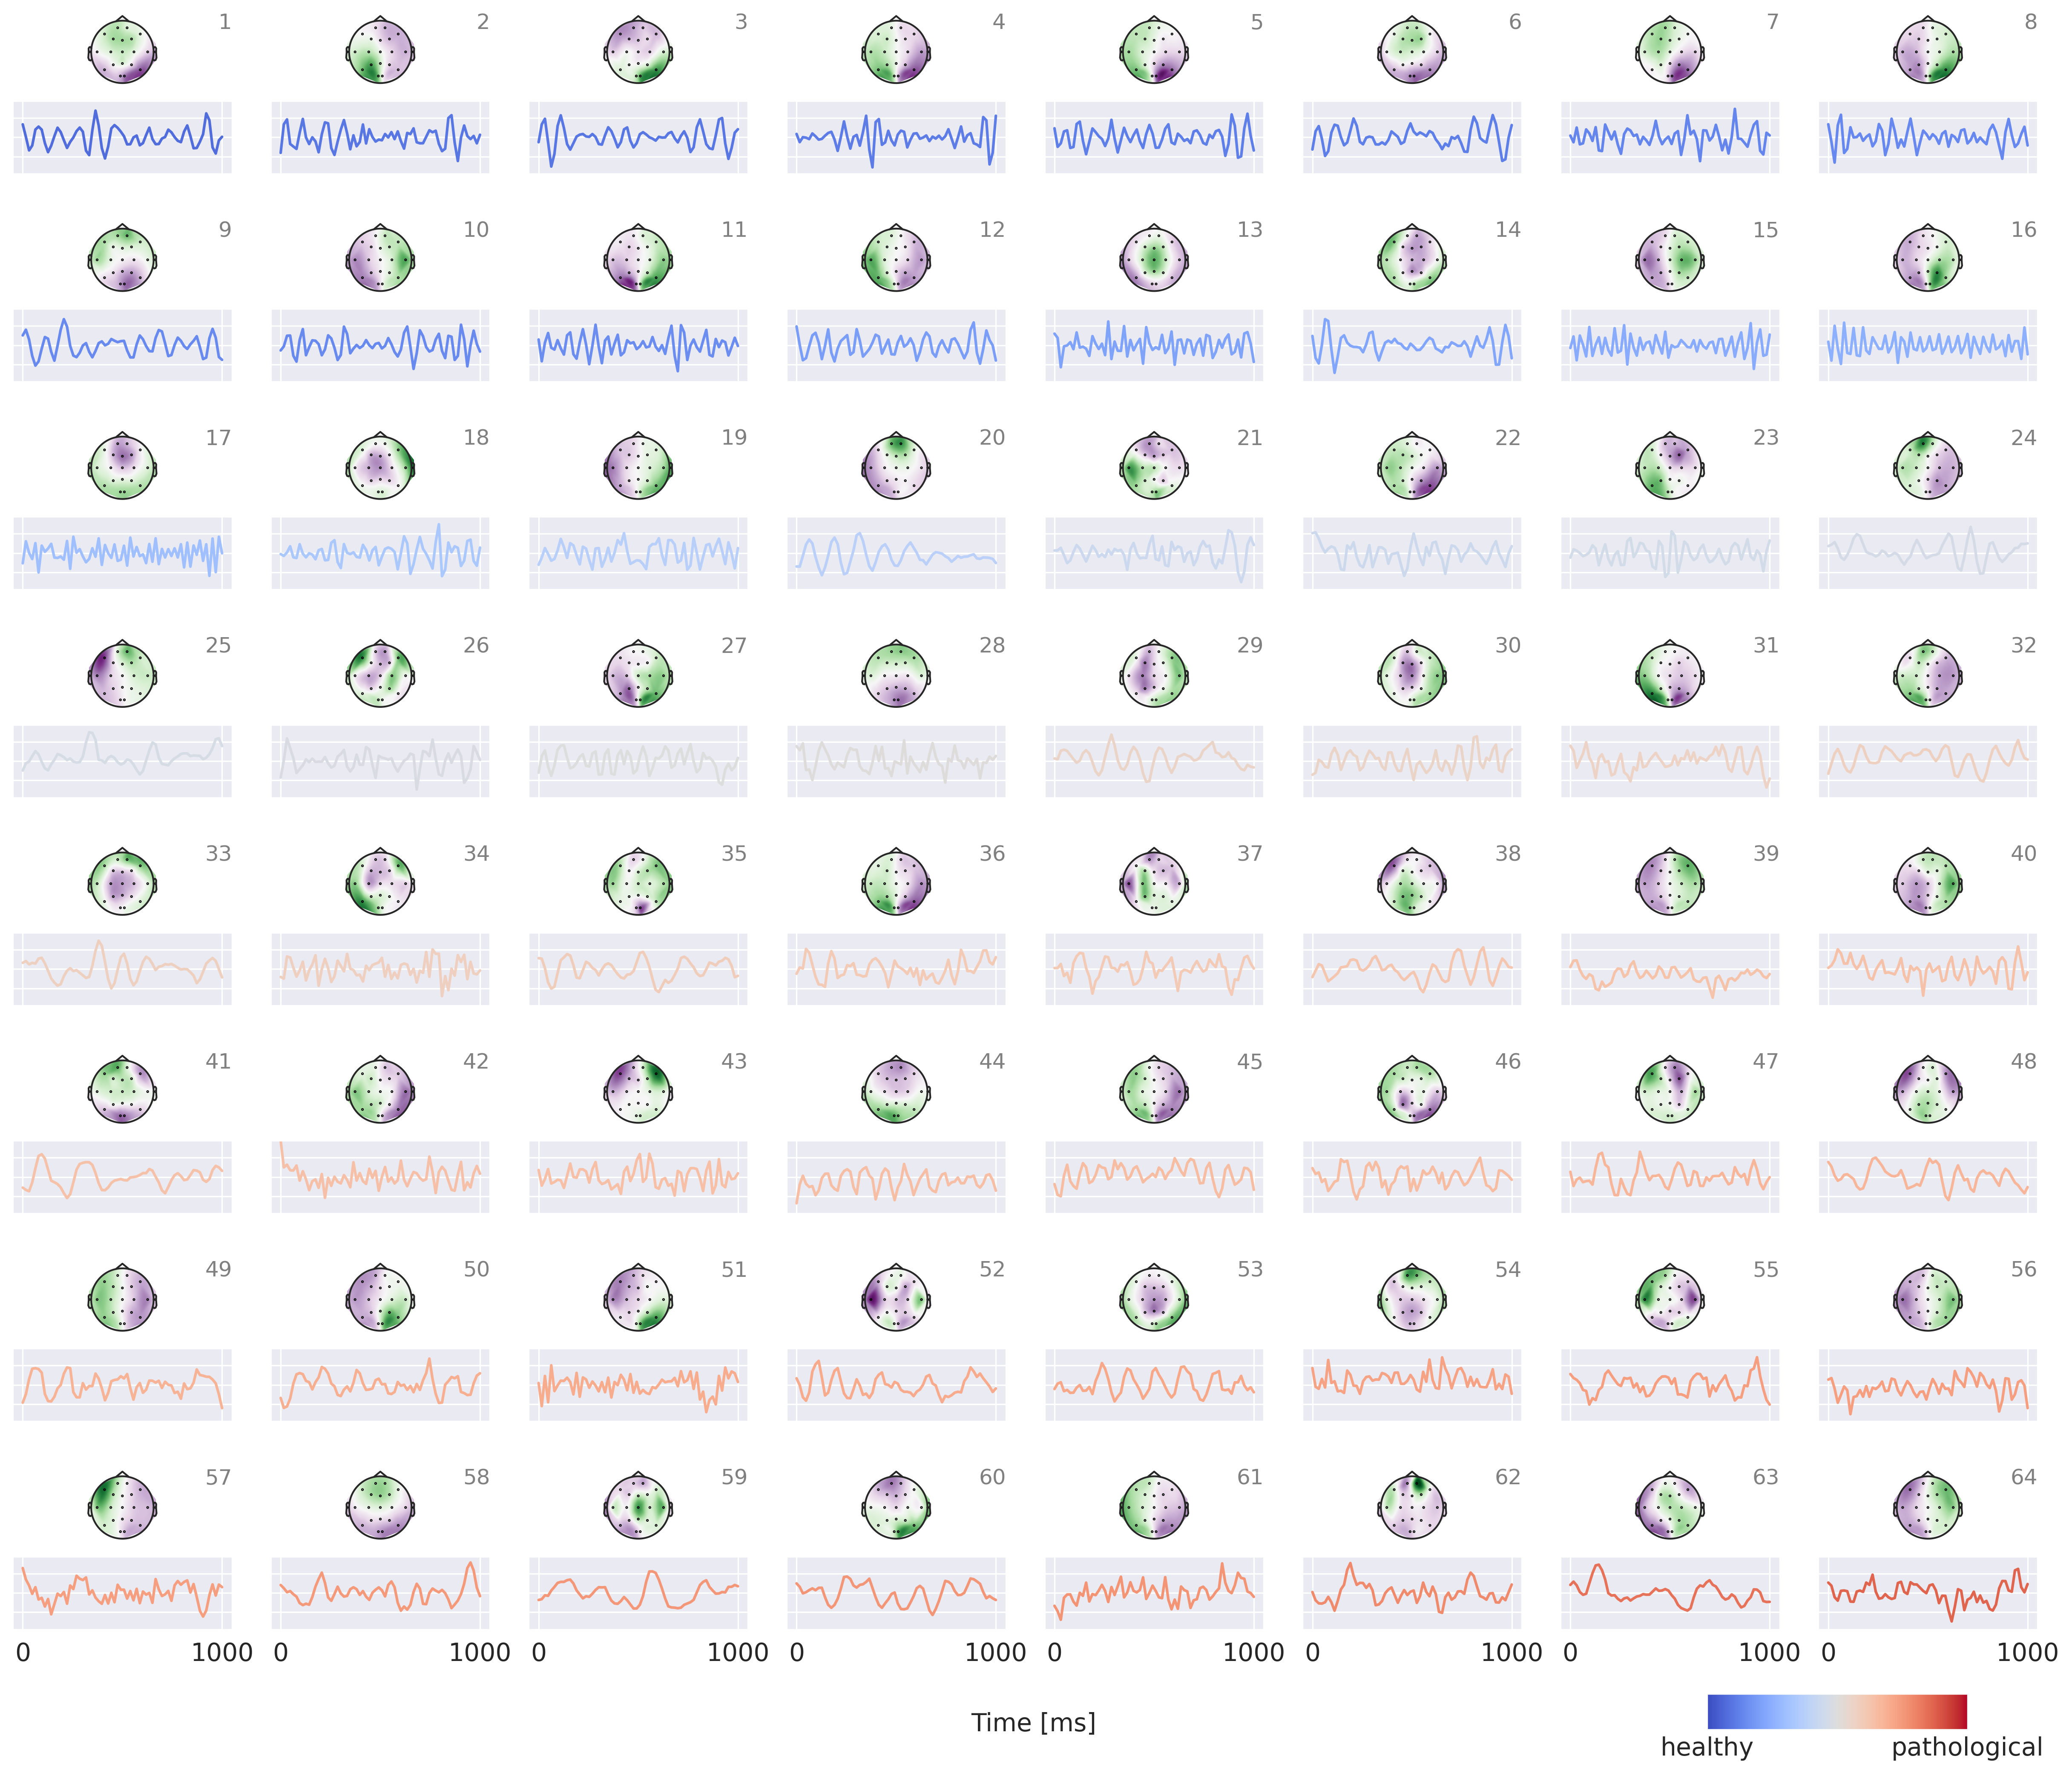
\includegraphics[width=1\linewidth]{images/cos-sim-net-pattern-with-hspace.png}
    \caption[Visualization of EEG-CosNet on pathology decoding]{
\textbf{Visualization of small interpretable EEG-CosNet trained to mimic
the EEG-InvNet.} Scalp Plots are spatial filter weights transformed to
patterns, signals below each scalp plot show corresponding convolutional
filter. Signal colors represent the weights of the linear classification
layer, transformed to patterns (see \Cref{methods-eeg-cosnet}
for an explanation). Plots are sorted by these colors. Note that
polarities of the scalp plots and temporal waveforms are arbitrary as
absolute cosine similarities are computed on the spatially filtered and
temporally convolved signals.
}
\label{cos-pattern}
\end{figure}

    Results for the EEG-CosNet show that a large fraction of the predictions
of the invertible network can be predicted from a relatively small
number of mostly neurophysiologically plausible spatio-temporal
patterns. EEG-CosNet predicts 88.8\% of the recordings in the same way
as the EEG-InvNet and retains a test set label accuracy of 82.6\% (see
\Cref{table-tuh-cos-net-accuracy}. This shows that from just
64 spatiotemporal features, the EEG-CosNet is able to predict the vast
majority of the EEG-InvNet predictions. Still, the remaining gap
indicates that the EEG-InvNet has learned some features that the
EEG-CosNet cannot represent.

Visualizations in \Cref{cos-sim-net-pattern-fig} show more
regular waveforms in the alpha and beta-frequency ranges with higher
association for the healthy class and more waveforms in other frequency
ranges as well as less regular waveforms with higher association for the
pathological class. As examples for the healthy class, plots 1 and 3
show oscillations with a strong alpha component and plots 15-17 show
oscillations with strong beta components. For the pathological class, we
see slower oscillations, e.g., in plots 53 and 60, and also more
irregular waveforms in, e.g., plots 49 and 52.

\section{Investigation of Very Low Frequencies}\label{investigation-of-very-low-frequencies}

    One surprising observation from the visualizations are differences in
the very low frequencies (\textless=0.5 Hz) between the two class
prototypes. For example, the very different mean values in the class
prototypes for FP1 and FP2 suggest very low frequency information
differs between the two classes on those electrodes. These kinds of
differences motivated us to more deeply investigate in how far very low
frequency information is predictive of pathology.



\begin{table}[h!tb]
    \myfloatalign
    \begin{tabularx}{\textwidth}{p{0.3\textwidth}p{0.3\textwidth}p{0.3\textwidth}}
    \toprule
        \tableheadlinewithwidth{0.3\textwidth}{EEG-InvNet}&
        \tableheadlinewithwidth{0.3\textwidth}{EEG-CosNet} &
        \tableheadlinewithwidth{0.3\textwidth}{Fourier-GMM} \\ 
        \midrule
        75.4 & 75.0 & 75.4 \\
        \bottomrule
    \end{tabularx}
    \caption[TUH test accuracy on lowpassed data]{
    \textbf{Test accuracy on data lowpassed below 0.5 Hz.} 
    }  \label{table-tuh-low-freq-accuracy}
\end{table}


    For this, we trained an EEG-InvNet on data lowpassed to be below 0.5 Hz.
For the lowpass, we first removed all Fourier components above 0.5 Hz
for each recording and also for each 2-second input window for the
network. This retained 75.4\% accuracy with the EEG-InvNet, indicating
even these very low frequencies remain fairly informative about the
pathologicality of the recording. We additionally trained the EEG-CosNet
with a temporal filter spanning the entire input window length of 2
seconds and found it to retain 75\% test accuracy. Finally, we also
directly trained a 8-component gaussian mixture model Fourier-GMM in
Fourier space. Only 3 dimensions per electrode remain: real value of the
0-Hz component ( summed values of the input window) and real and
imaginary value of the 0.5-Hz Fourier component). Each of the 8 mixture
components had learnable class weights, how much each mixture component
contributed to that classes learned distribution. The Fourier-GMM also
retains 75.4\% test accuracy. All results are shown in
\Cref{table-tuh-low-freq-accuracy}.

\subsection{EEG-InvNet
Visualizations}\label{eeg-invnet-visualizations}

\begin{figure}[h!tb]
    \myfloatalign
    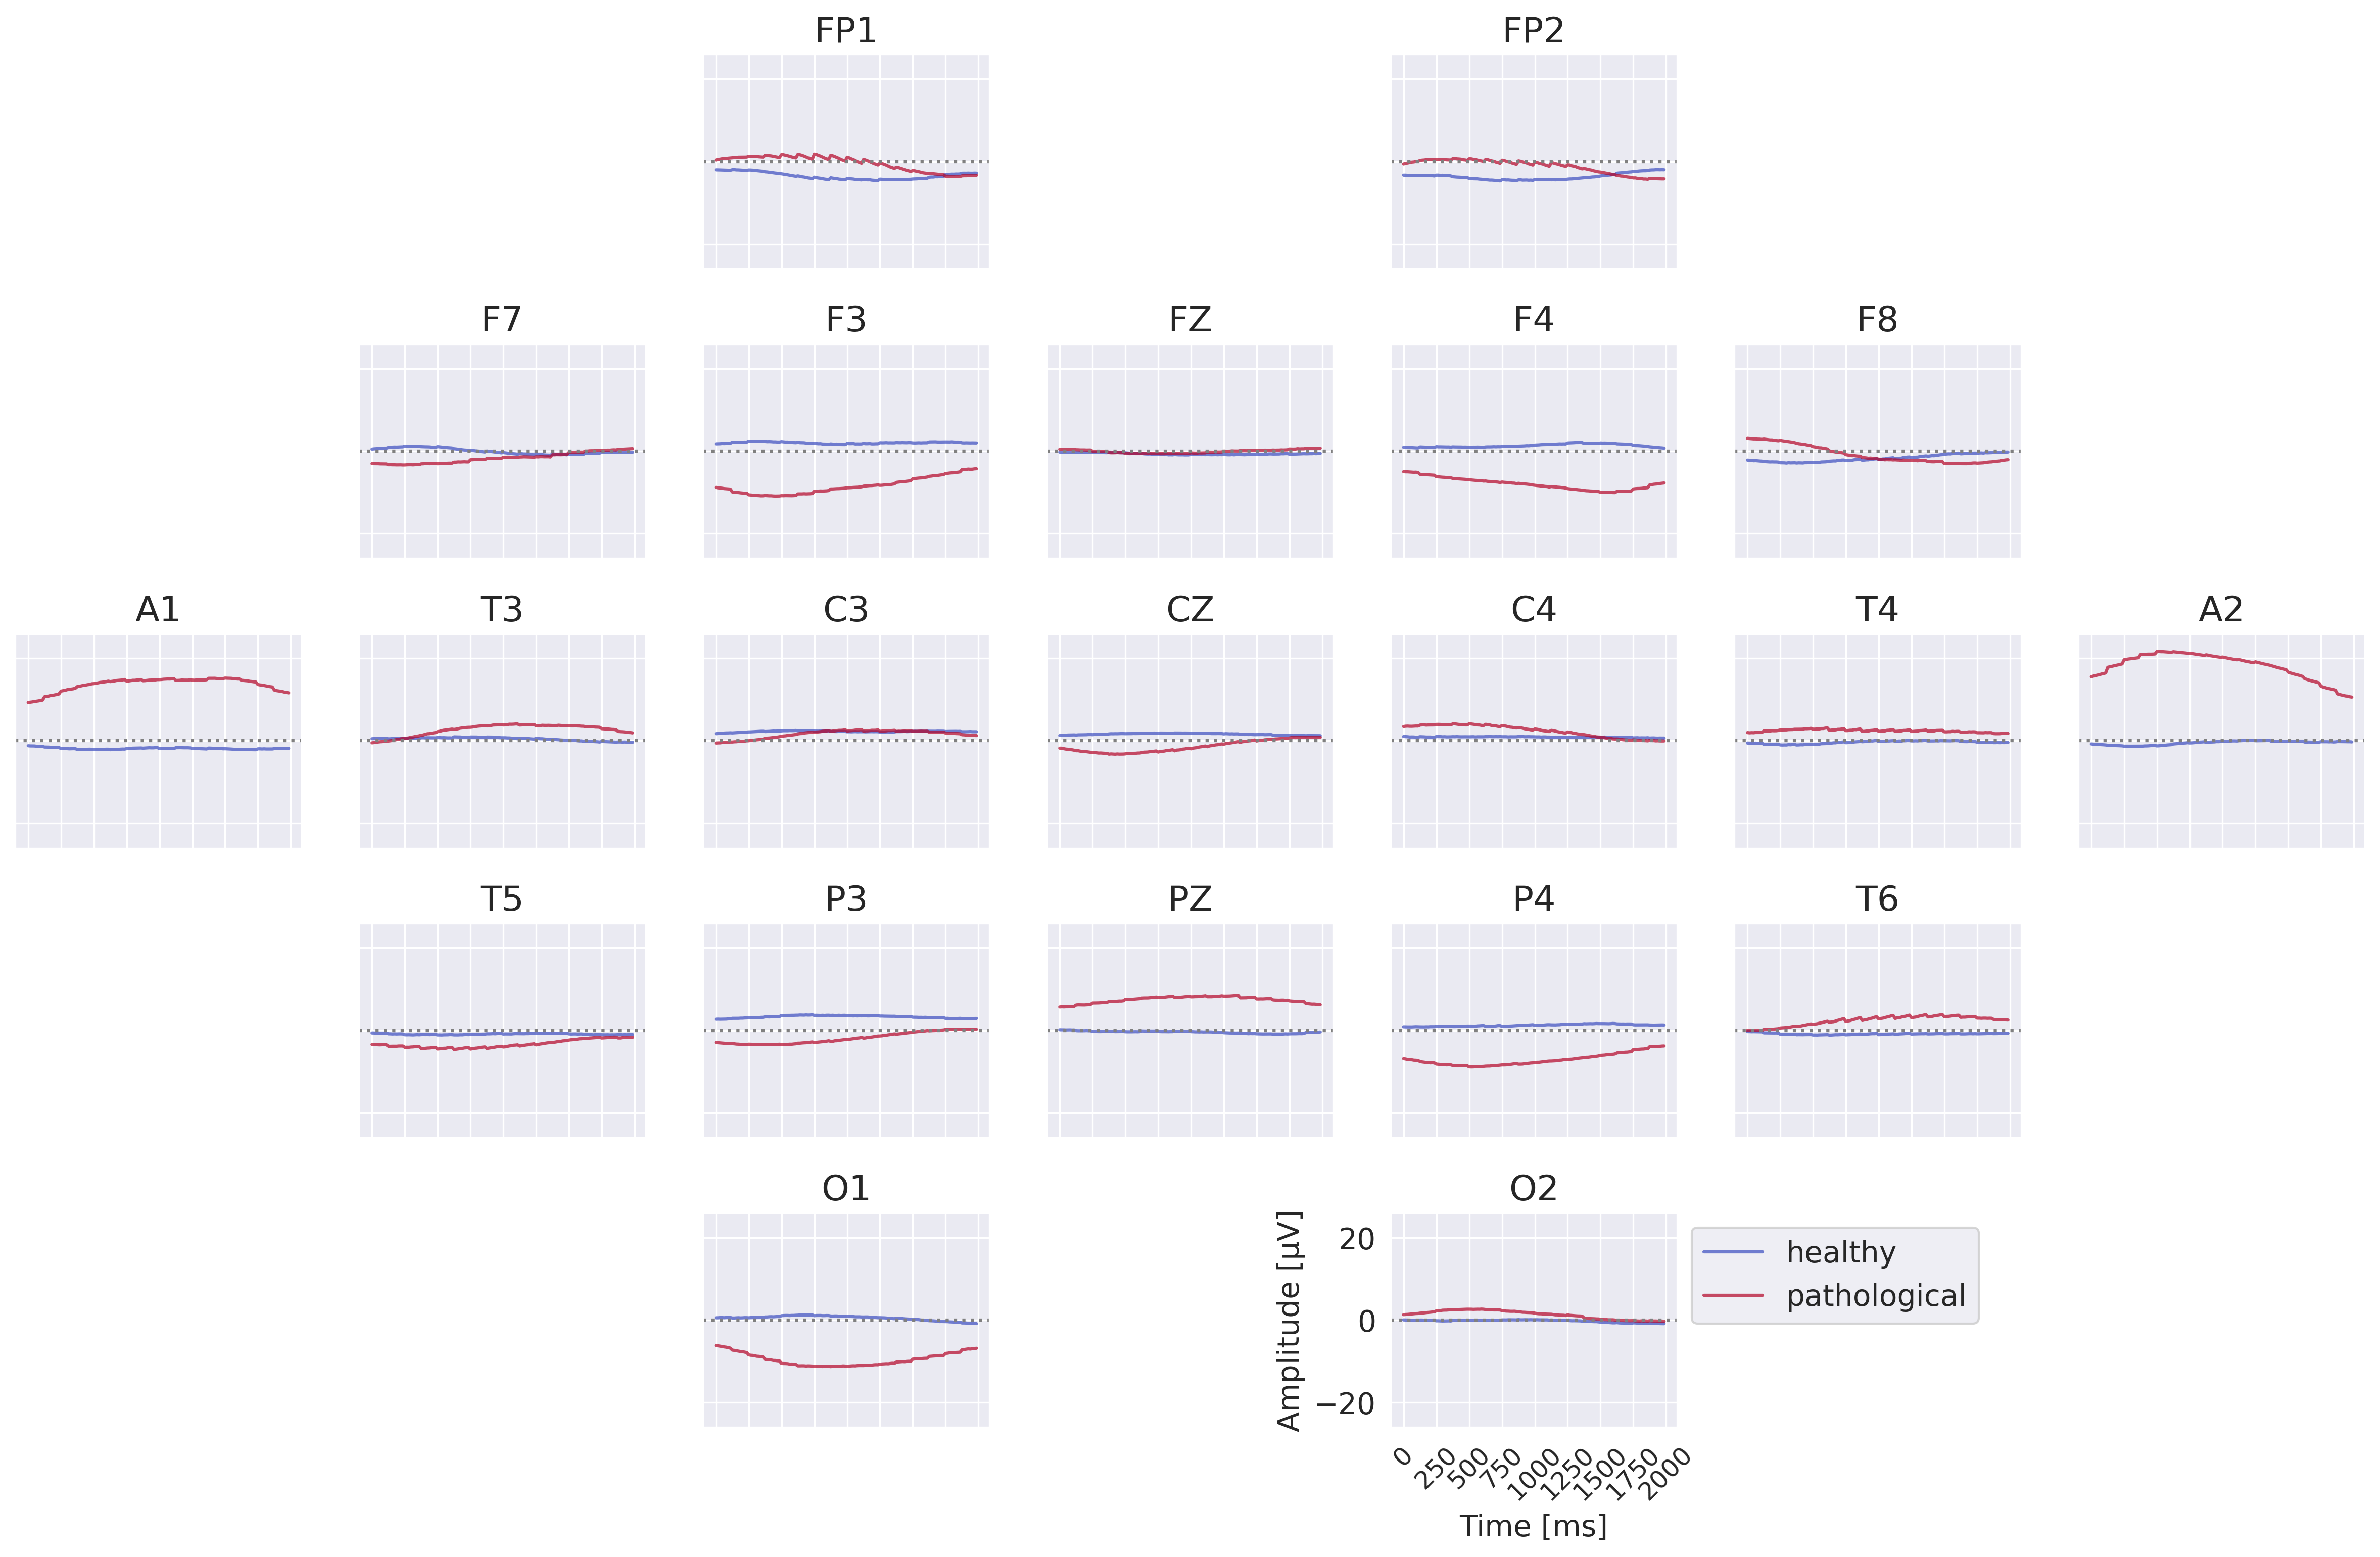
\includegraphics[width=.9\linewidth]{images/net-lowfreq-prototypes.png}
    \caption[EEG-InvNet low-frequency class prototypes]{
\textbf{Class prototypes for the EEG-InvNet trained on data lowpassed to
be below 0.5 Hz.} Note large differences at A1 and A2.
}
\label{net-low-freq-prototypes-fig}
\end{figure}


\begin{figure}[h!tb]
    \myfloatalign
    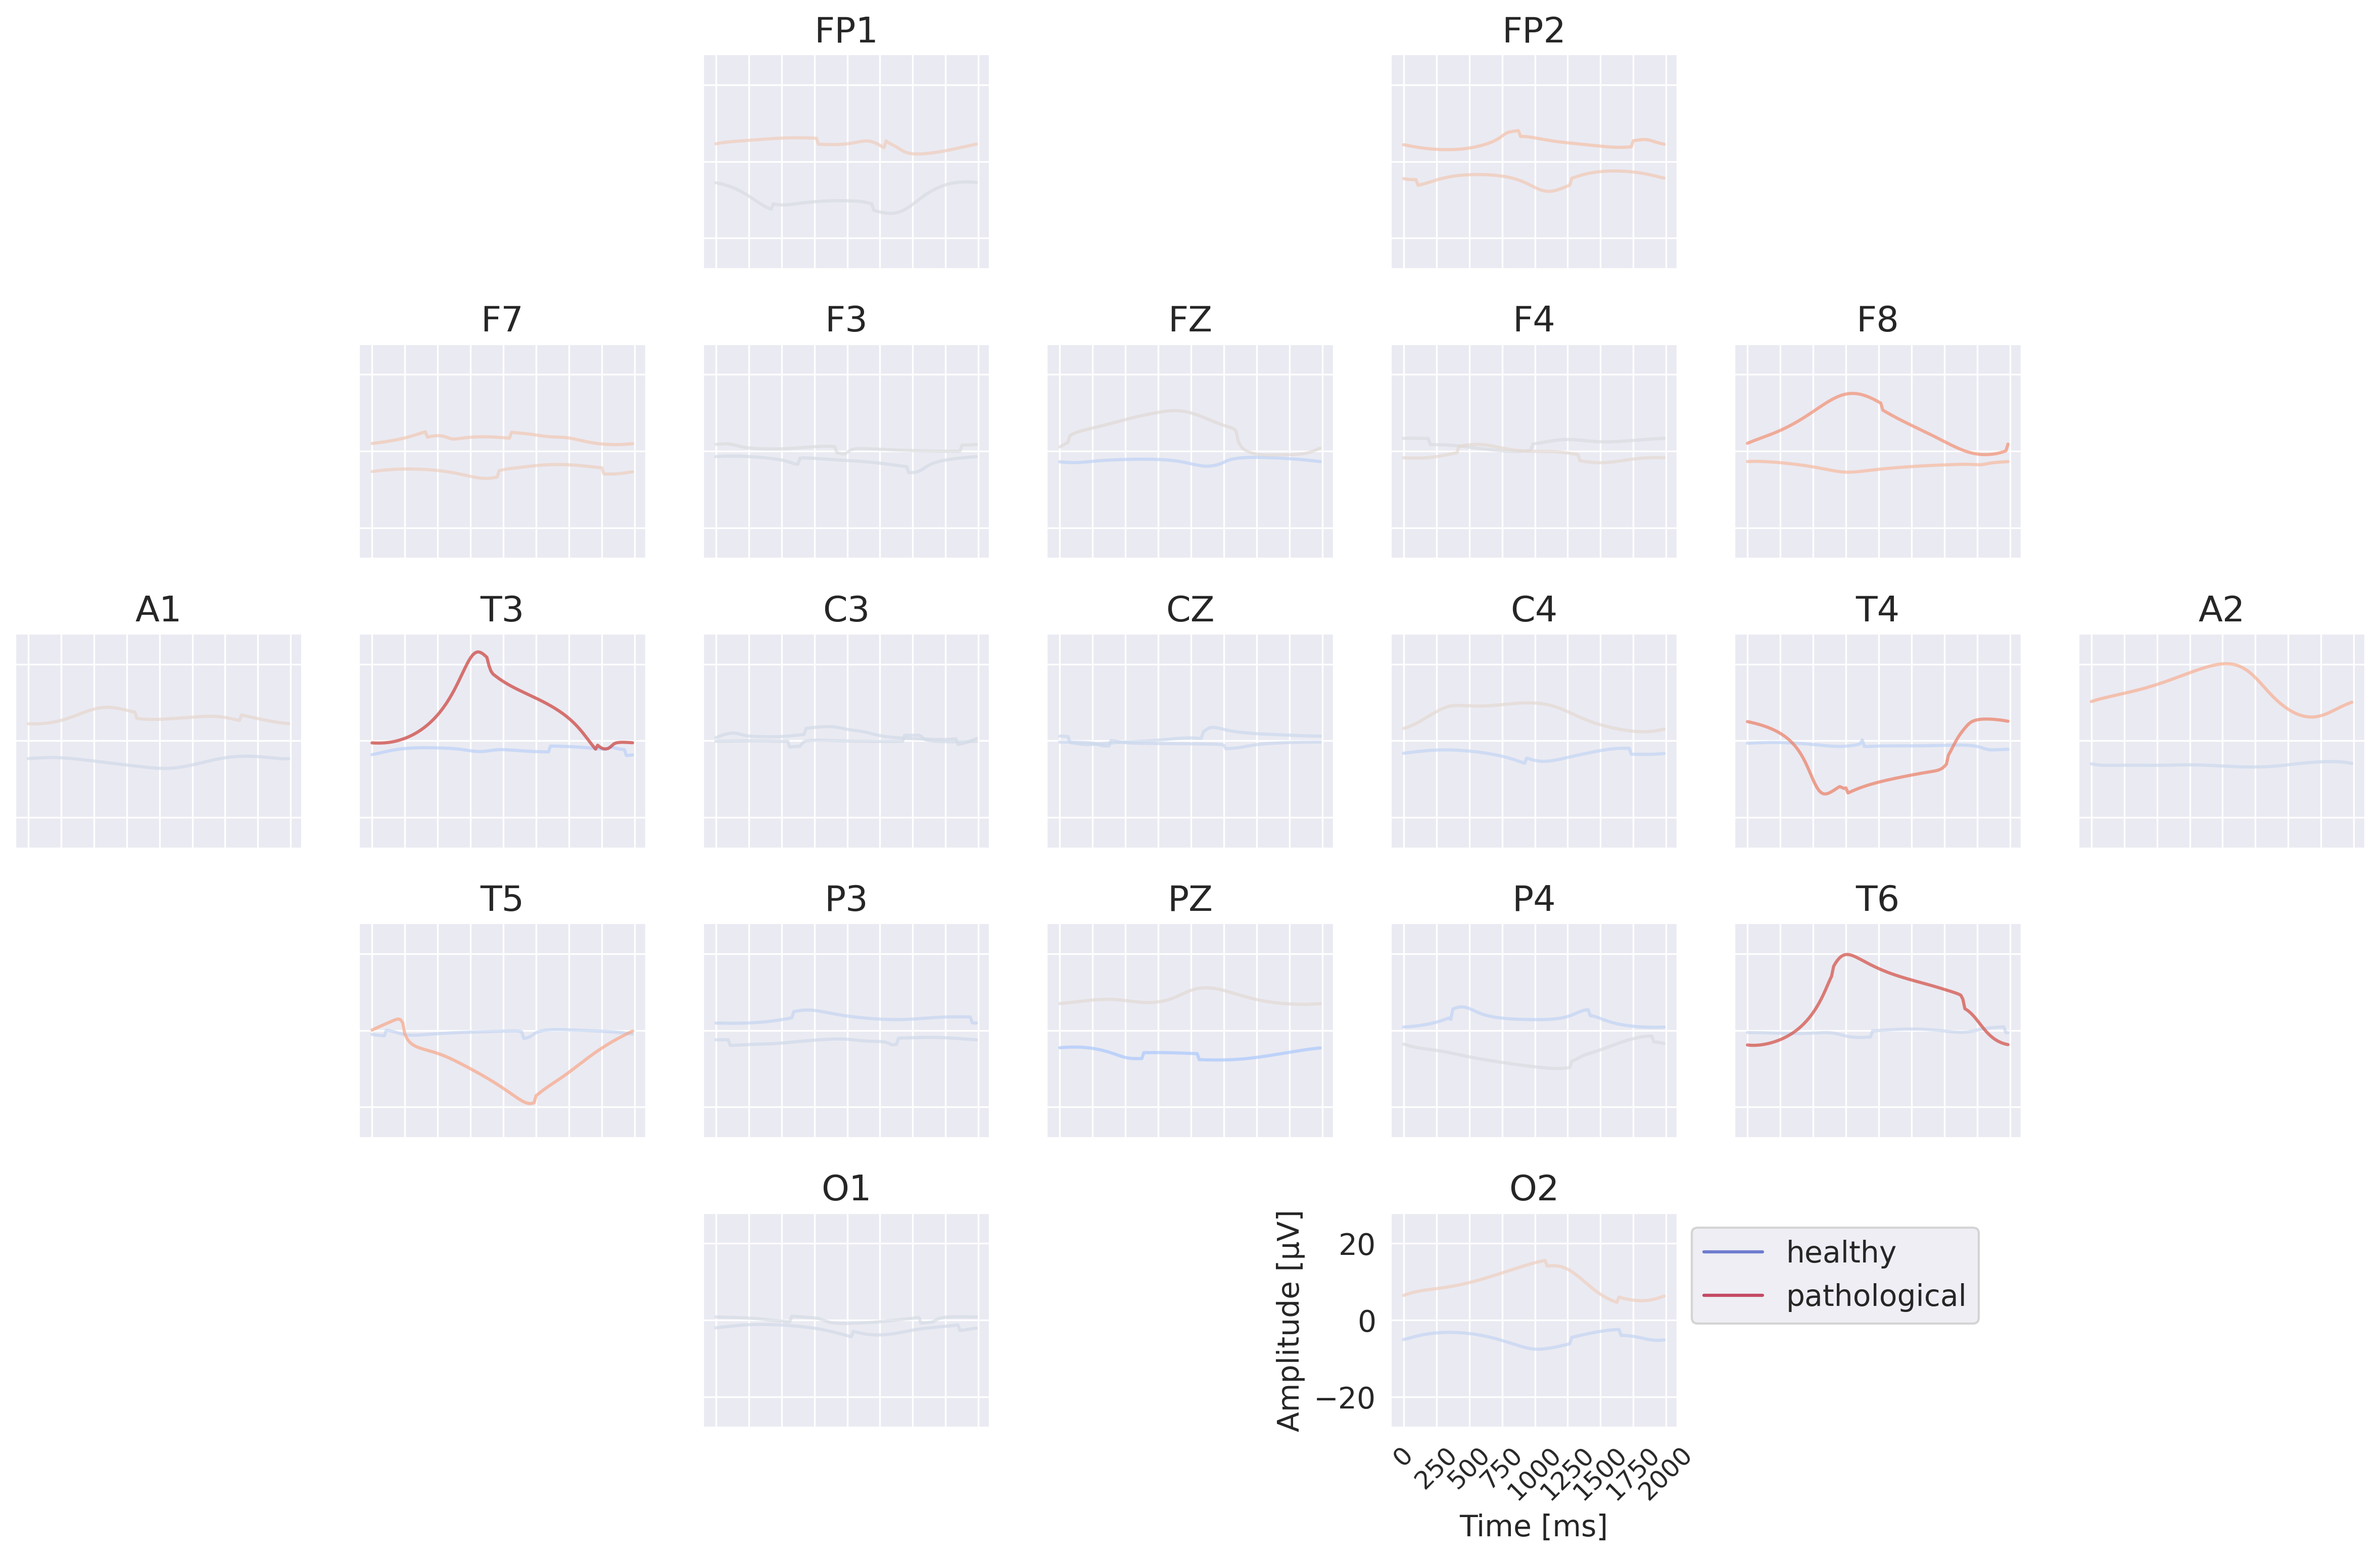
\includegraphics[width=.9\linewidth]{images/marginal-chan-low-freq.png}
    \caption[EEG-InvNet low-frequency class prototypes]{
\textbf{Per-electrode prototypes for EEG-InvNet trained on data
lowpassed below 0.5 Hz.} Note strongly predictive signals at T3,T4,T6.
}
\label{marginal-chan-low-freq}
\end{figure}


    The visualizations of the EEG-InvNet show several interesting features.
The class prototypes in \Cref{net-low-freq-prototypes-fig}
show differences at most electrodes, especially pronounced for A1 and
A2. The per-electrode prototypes in
\Cref{marginal-chan-low-freq} show predictive
information in the T3,T4 and T6 electrodes.


\subsection{EEG-CosNet
Visualizations}\label{eeg-cosnet-visualizations}

\begin{figure}[h!tb]
    \myfloatalign
    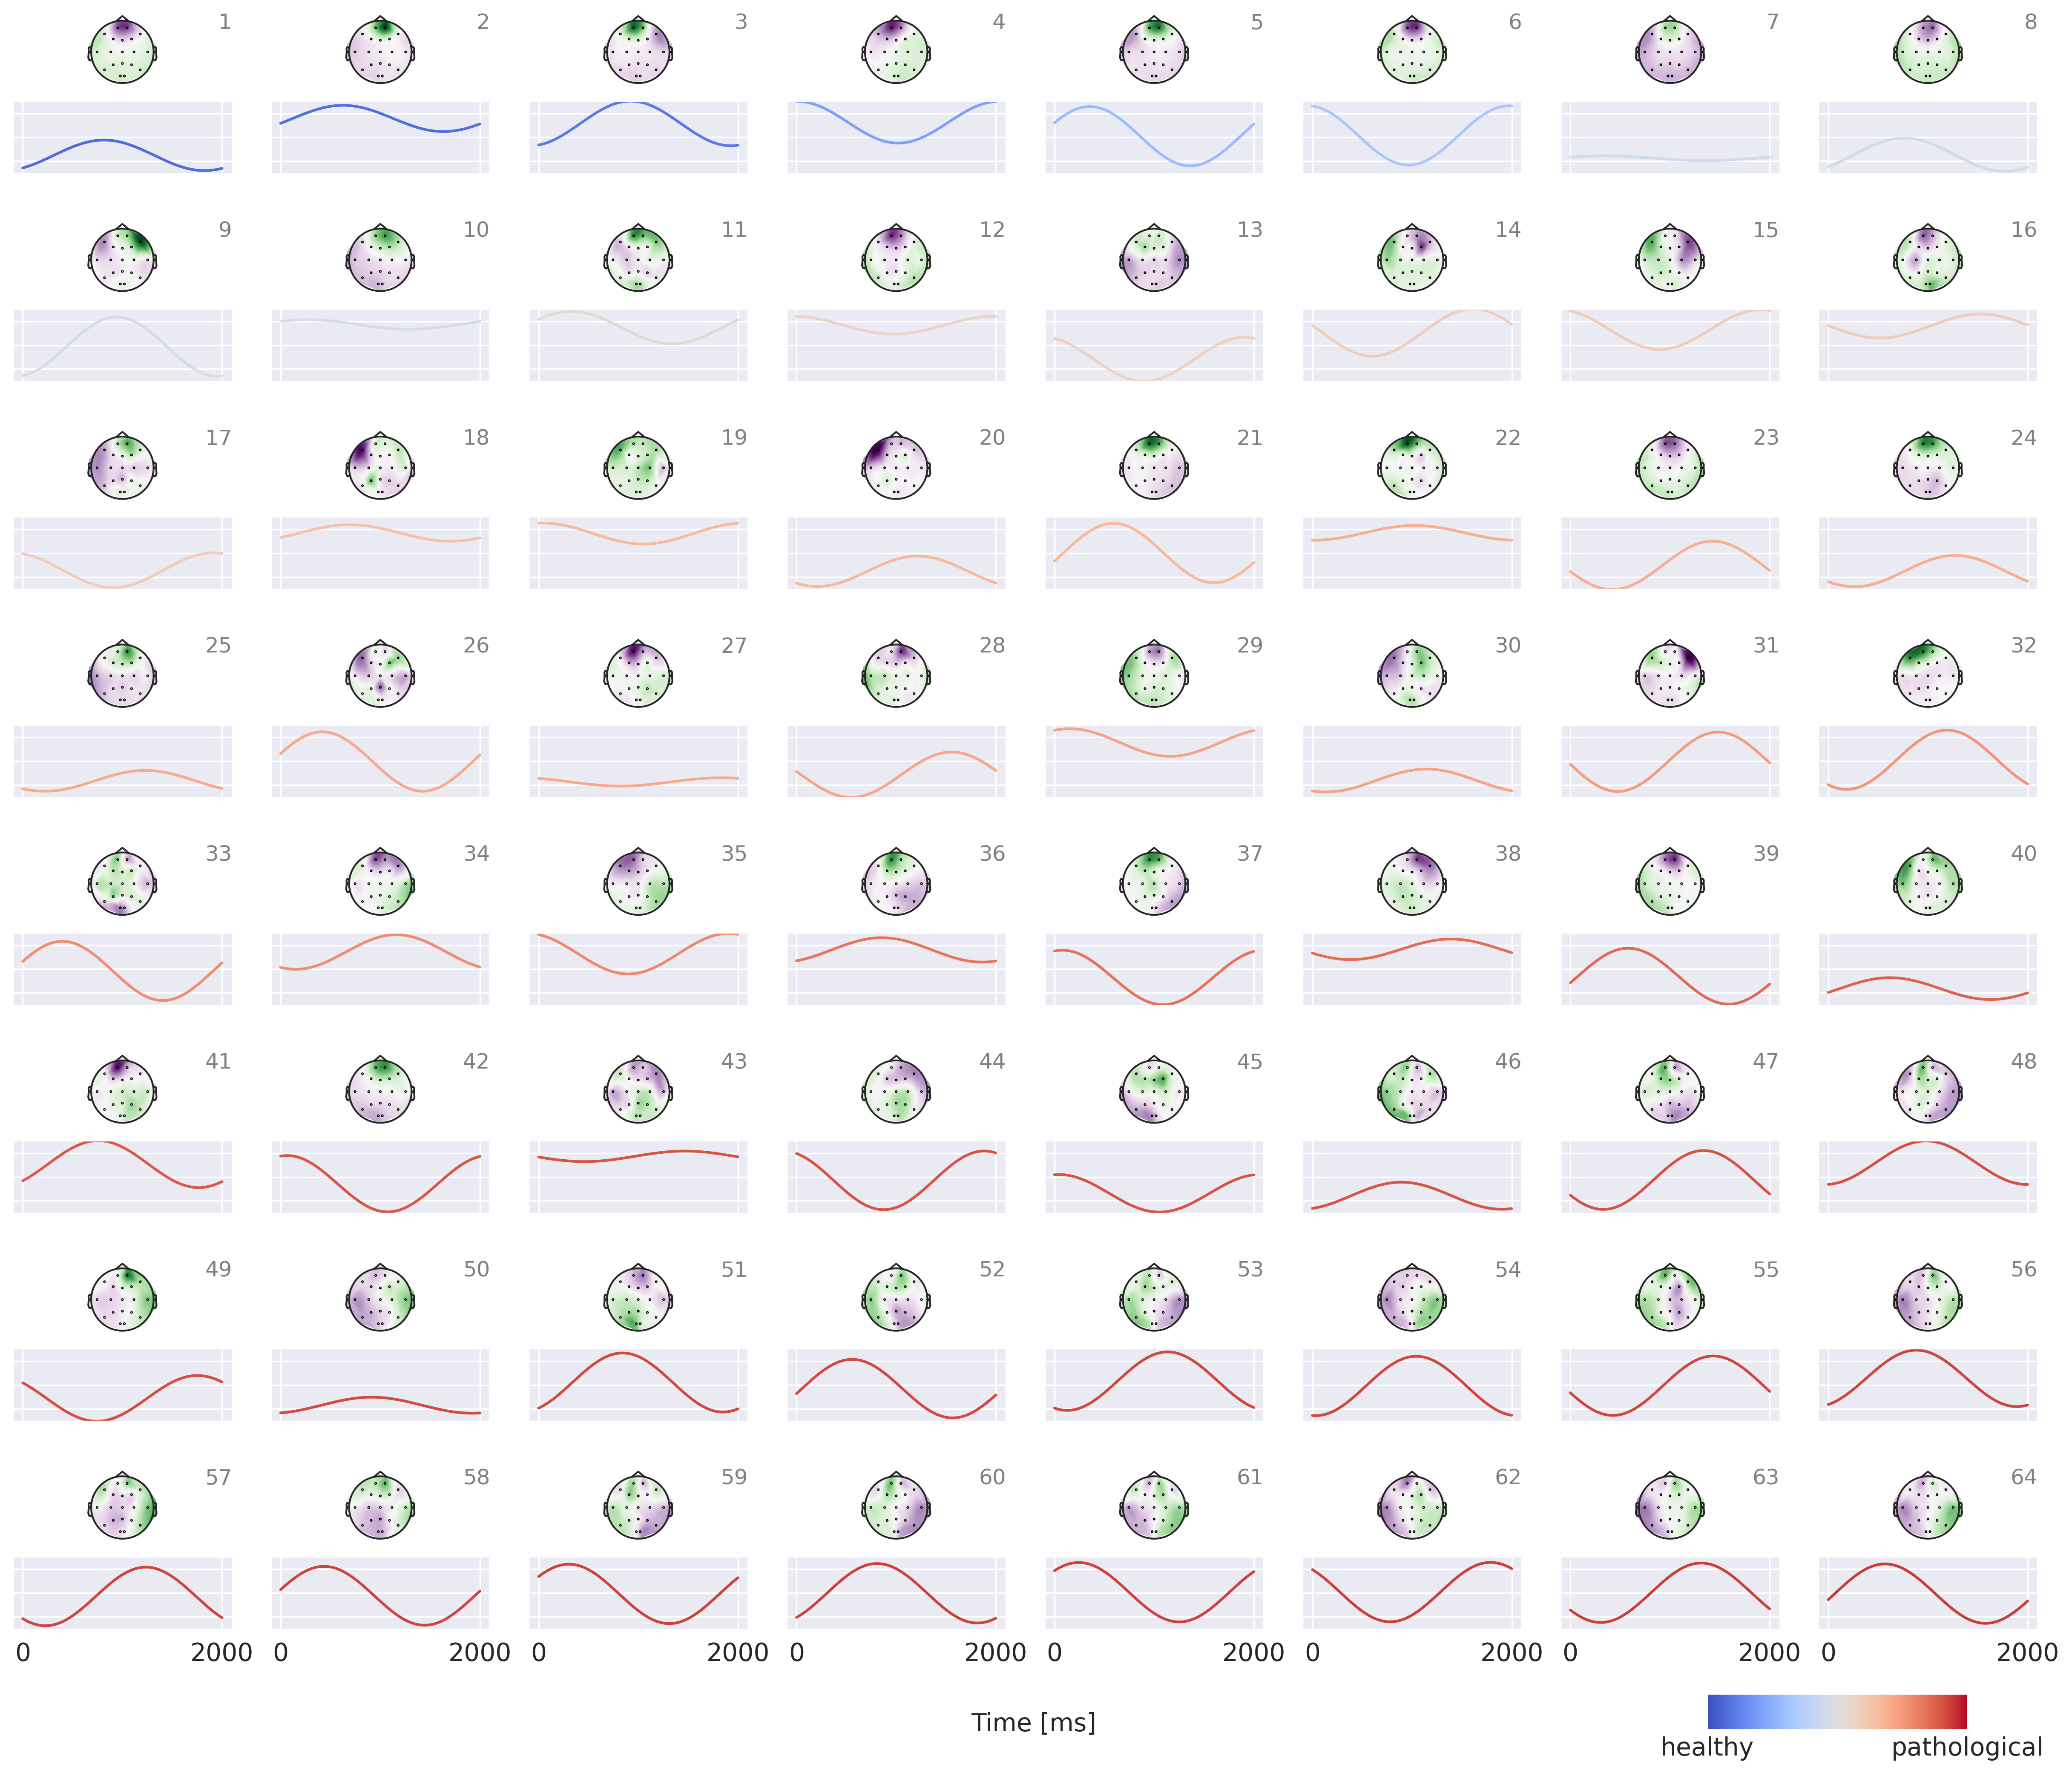
\includegraphics[width=1\linewidth]{images/cos-sim-net-low-freq-pattern-with-hspace.png}
    \caption[EEG-CosNet visualizations on lowpassed data]{
\textbf{Spatiotemporal patterns for EEG-CosNet trained on lowpassed data
below 0.5 Hz.} Note large frontal components associated with healthy
class.
}
\label{cos-sim-net-low-freq-pattern-fig}
\end{figure}


Visualization of the EEG-CosNet in
\Cref{cos-sim-net-low-freq-pattern-fig} contain strong
frontally components associated with the healthy class and components in
temporal areas associated with the pathological class. The temporal
components are in line with the per-electrode visualization, and the
frontal components were already visible as differences in mean signal
values in the class prototypes on the original data.


\subsection{Fourier-GMM
Visualizations}\label{fourier-gmm-visualizations}



\begin{figure}[h!tb]
    \captionsetup[subfigure]{labelformat=empty}
    \myfloatalign
    \subfloat[]
    {
    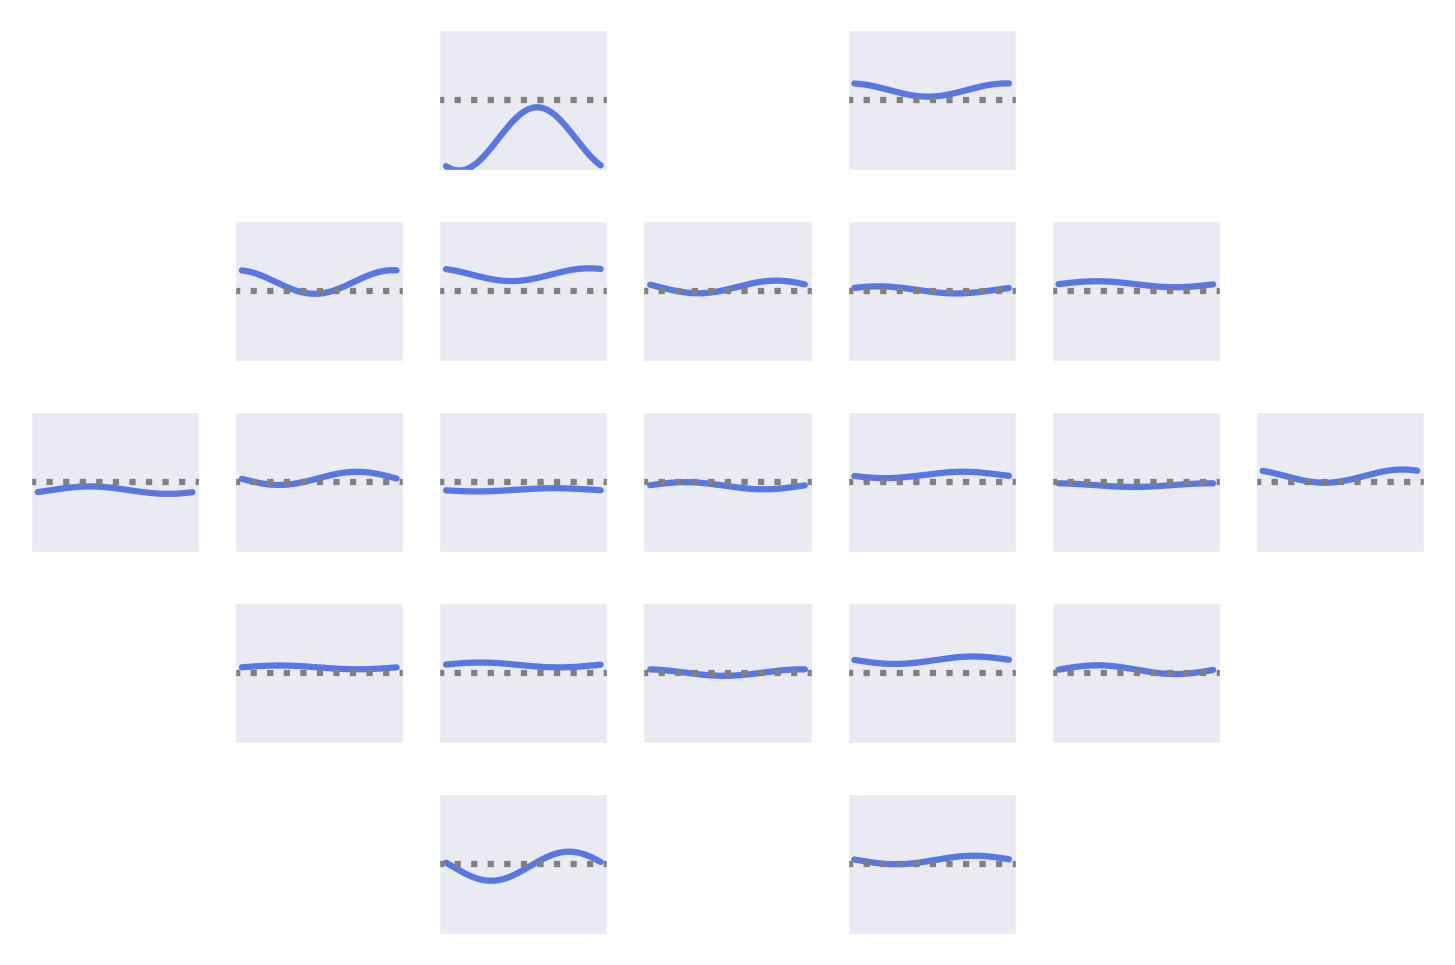
\includegraphics[width=.2\linewidth]{images/low-freq-prototypes-0.png}} \quad\subfloat[]
    {
    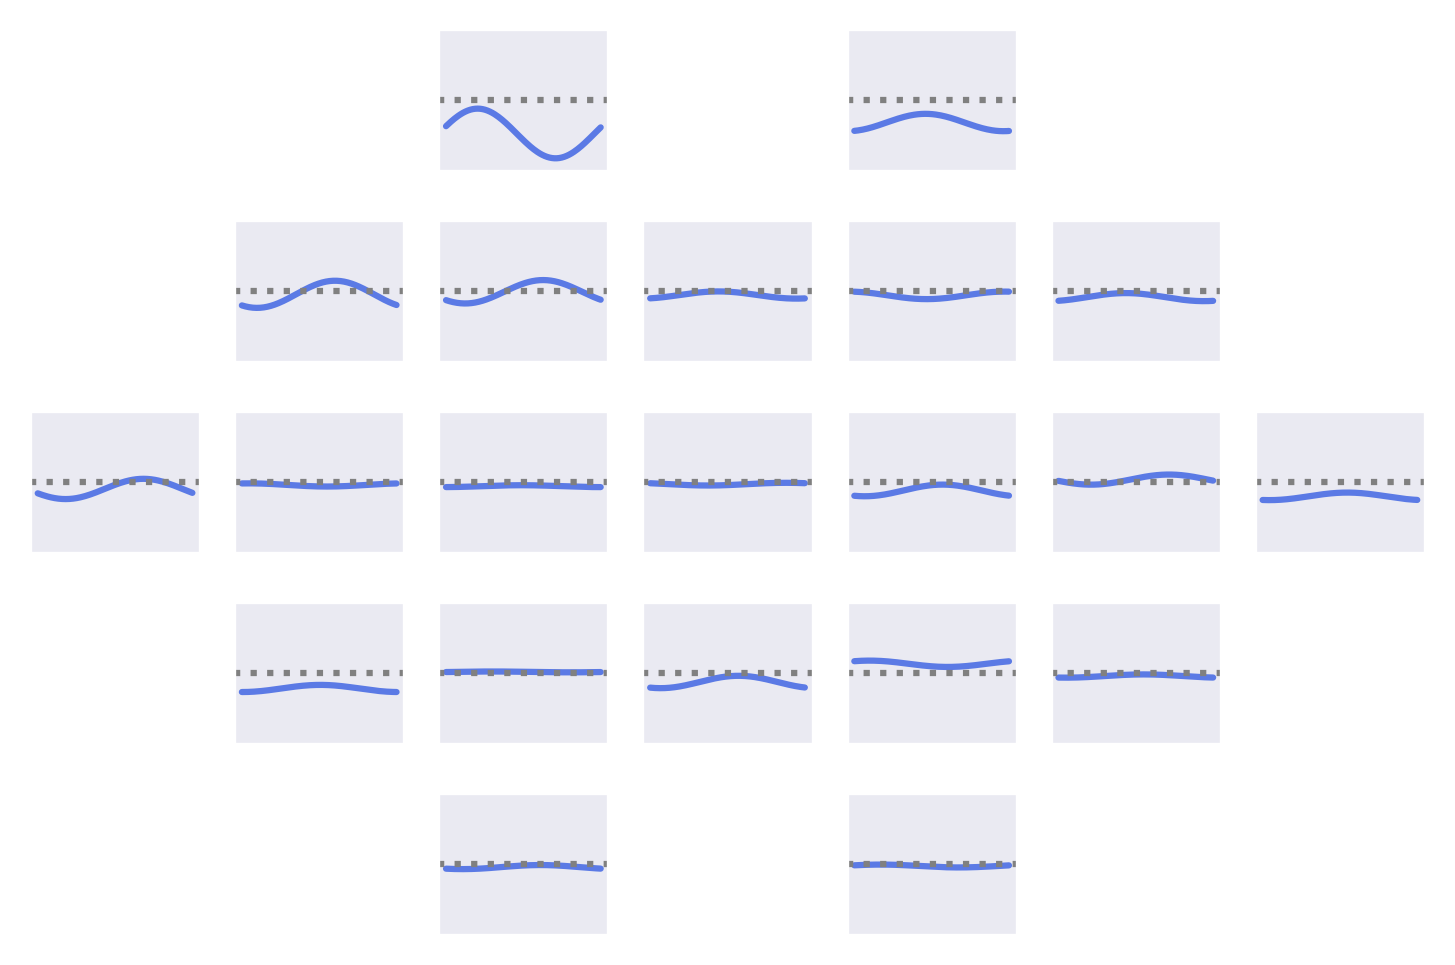
\includegraphics[width=.2\linewidth]{images/low-freq-prototypes-1.png}} \quad\subfloat[]
    {
    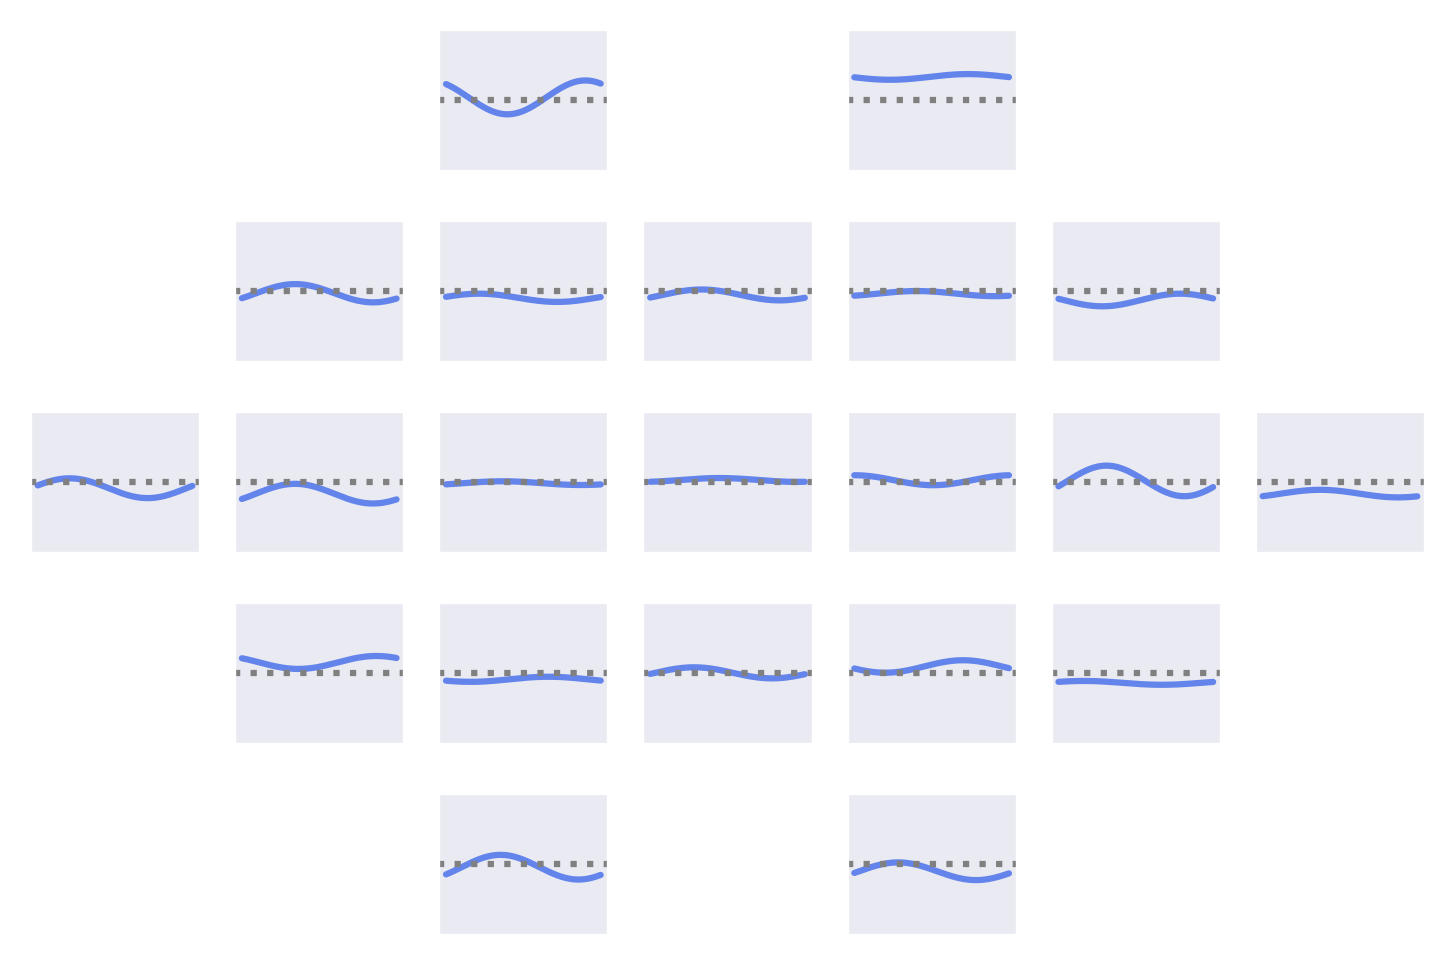
\includegraphics[width=.2\linewidth]{images/low-freq-prototypes-2.png}} \quad
    \subfloat[] 
    {
        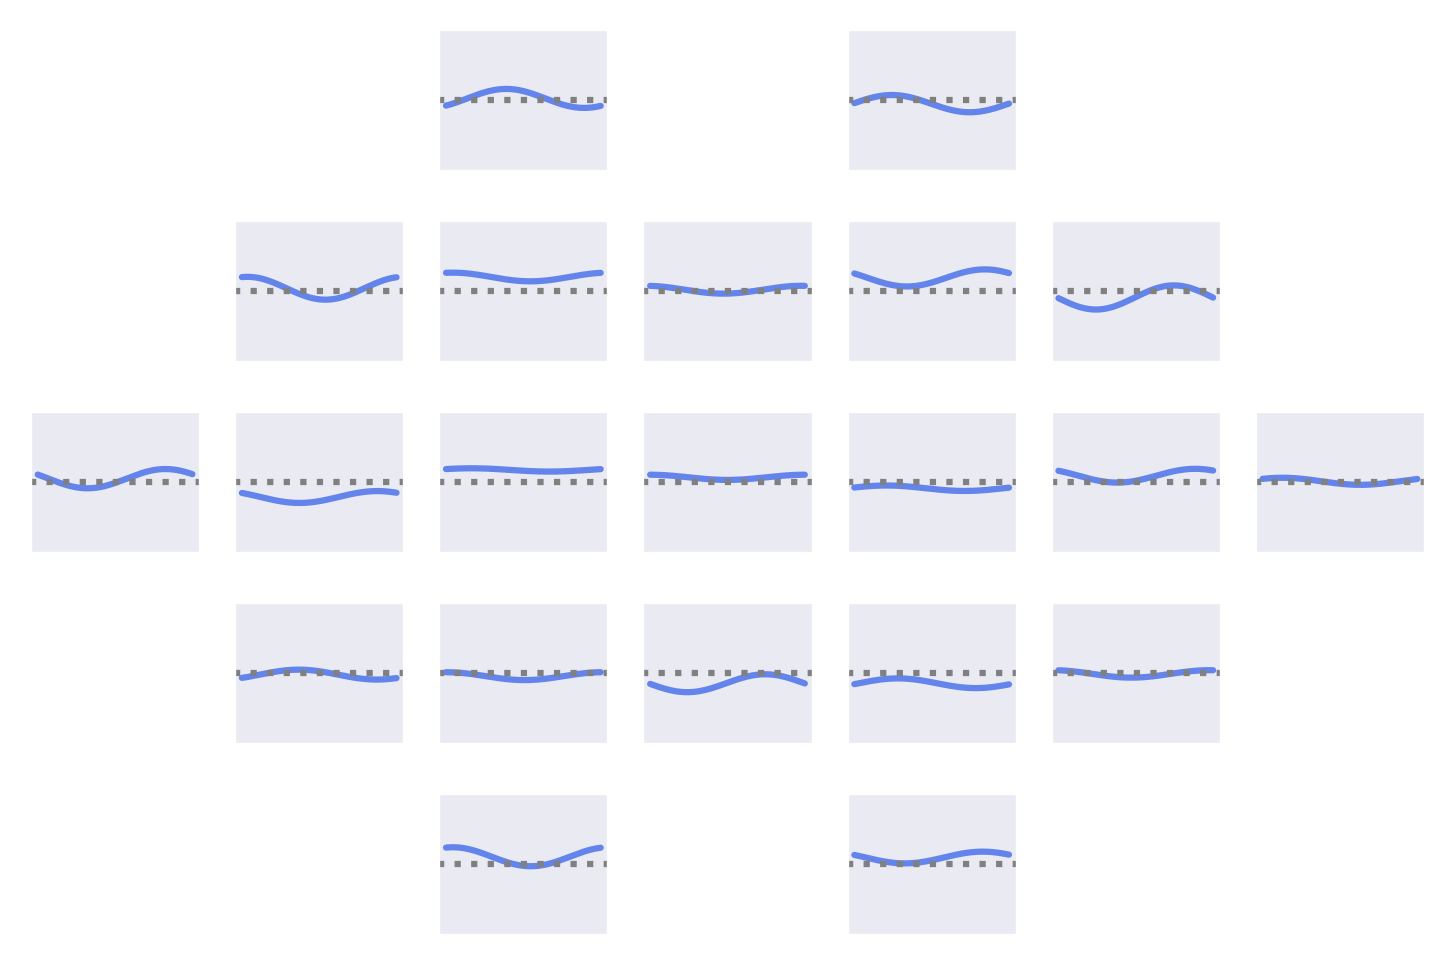
\includegraphics[width=.2\linewidth]{images/low-freq-prototypes-3.png}} \\
    \subfloat[]
    {
    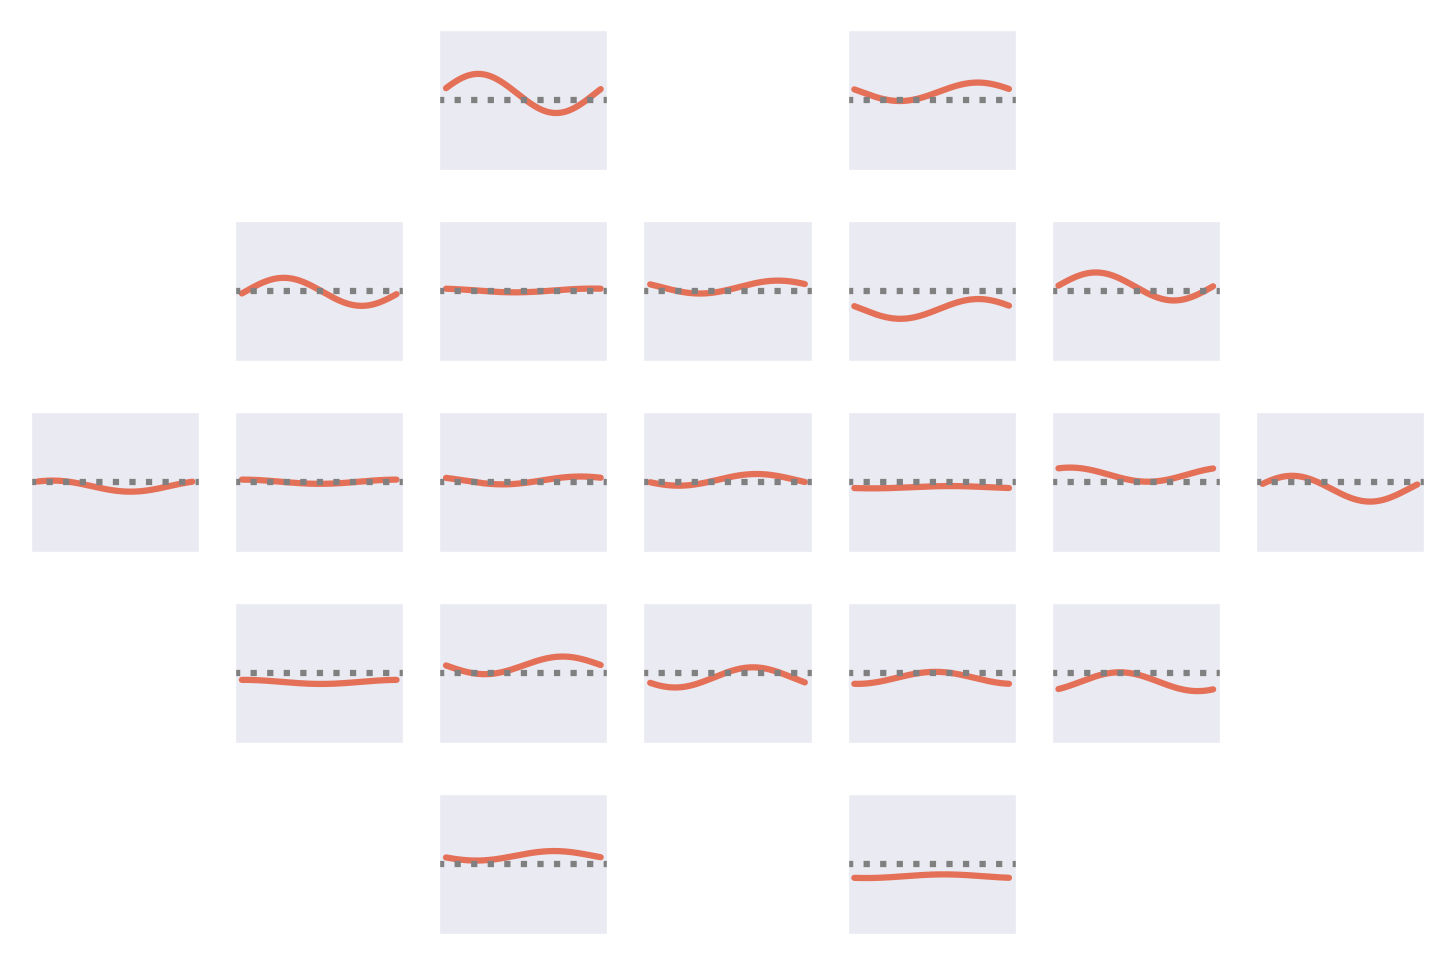
\includegraphics[width=.2\linewidth]{images/low-freq-prototypes-4.png}} \quad\subfloat[]
    {
    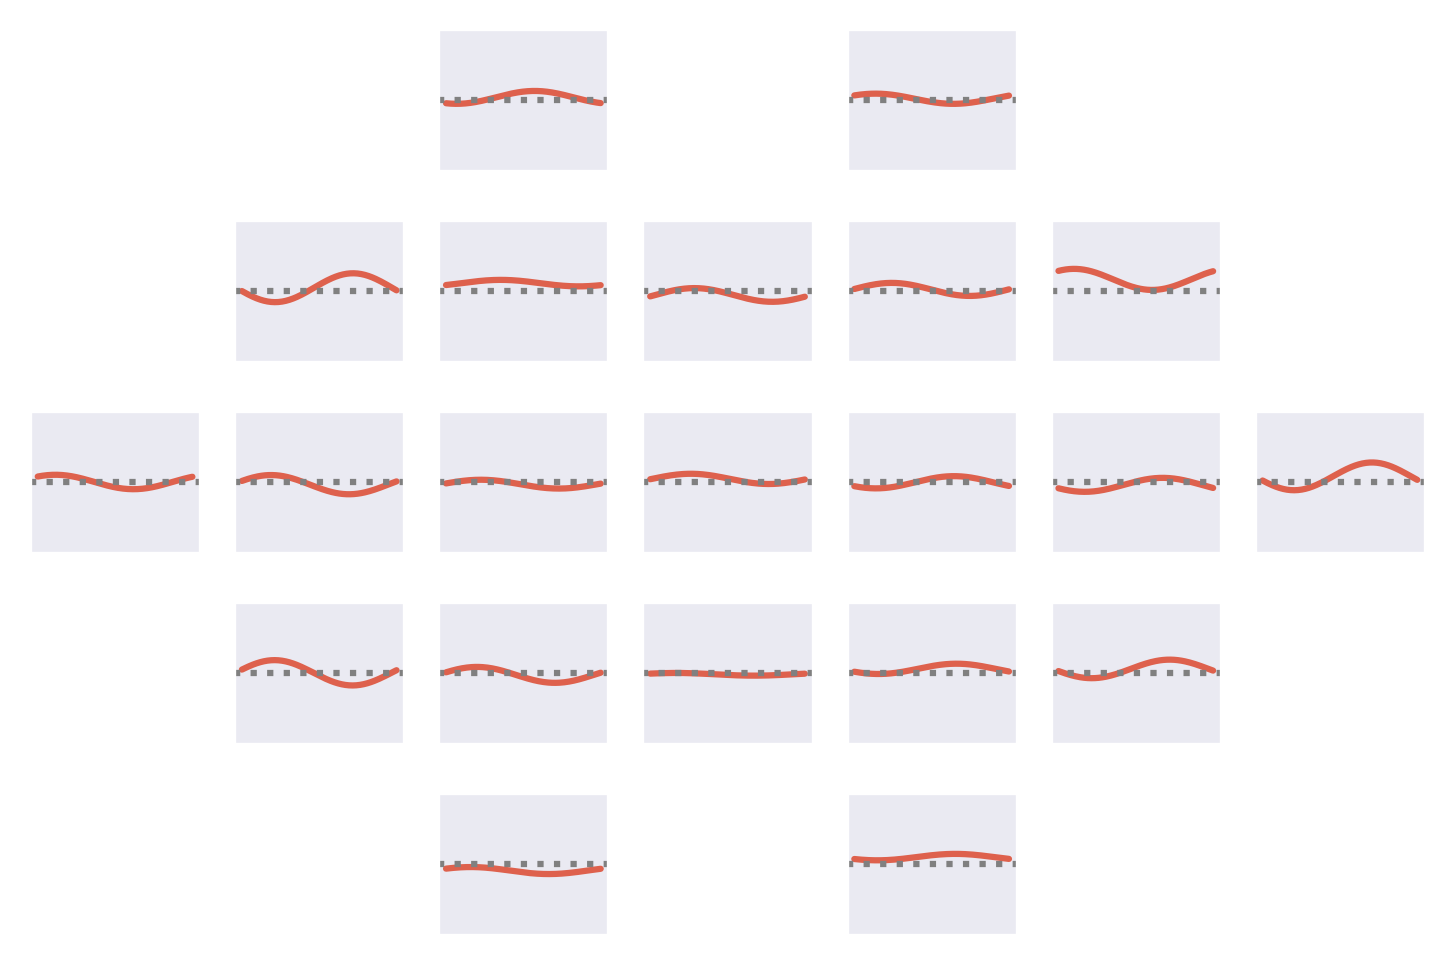
\includegraphics[width=.2\linewidth]{images/low-freq-prototypes-5.png}} \quad\subfloat[]
    {
    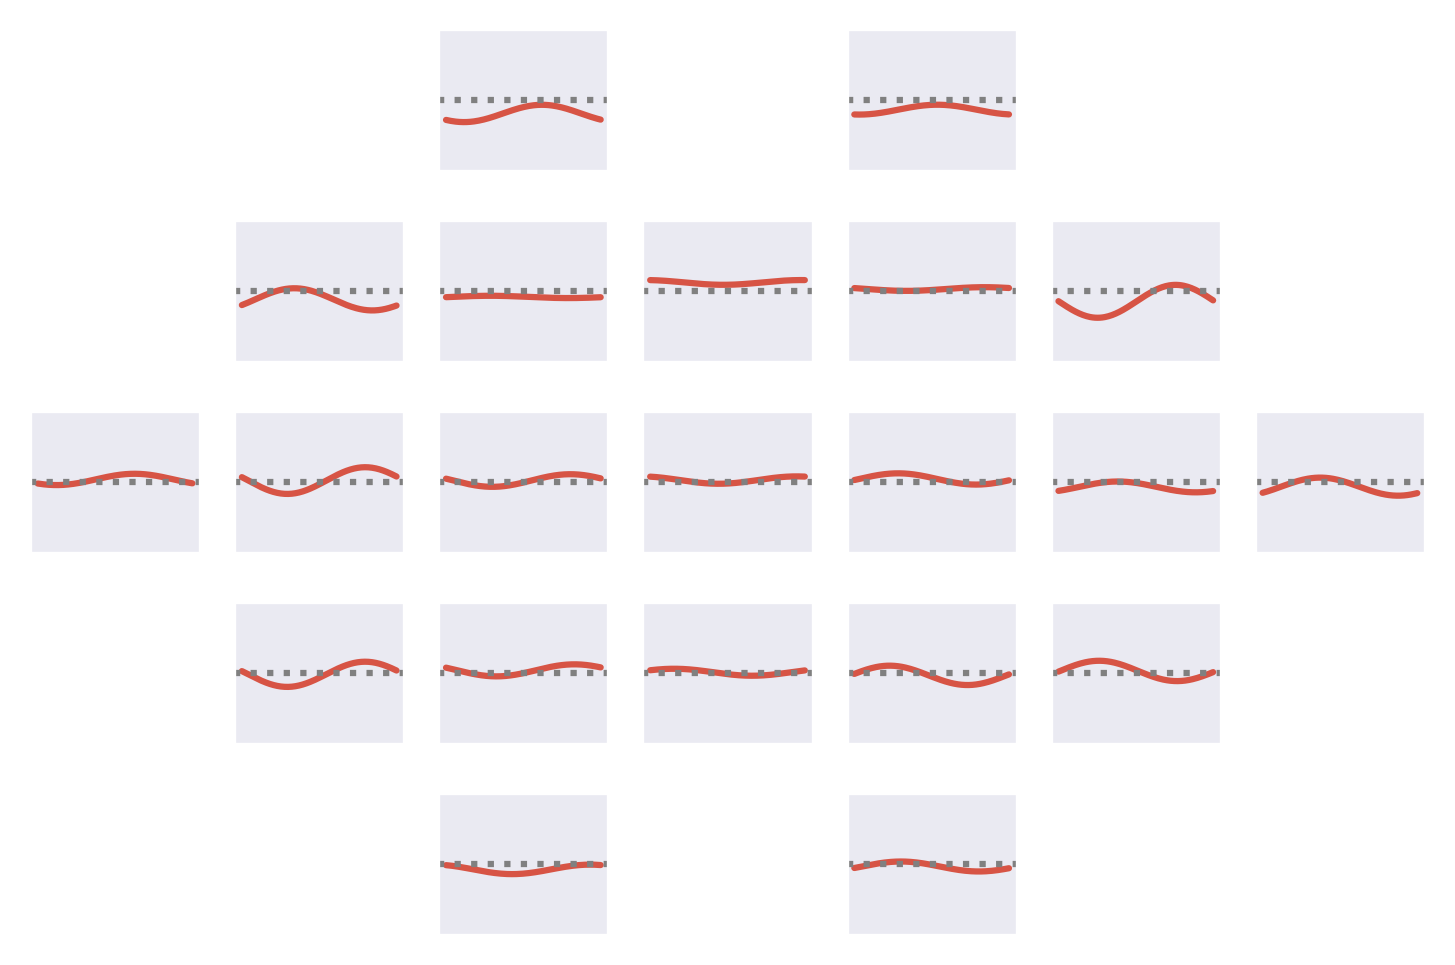
\includegraphics[width=.2\linewidth]{images/low-freq-prototypes-6.png}} \quad
    \subfloat[] 
    {
        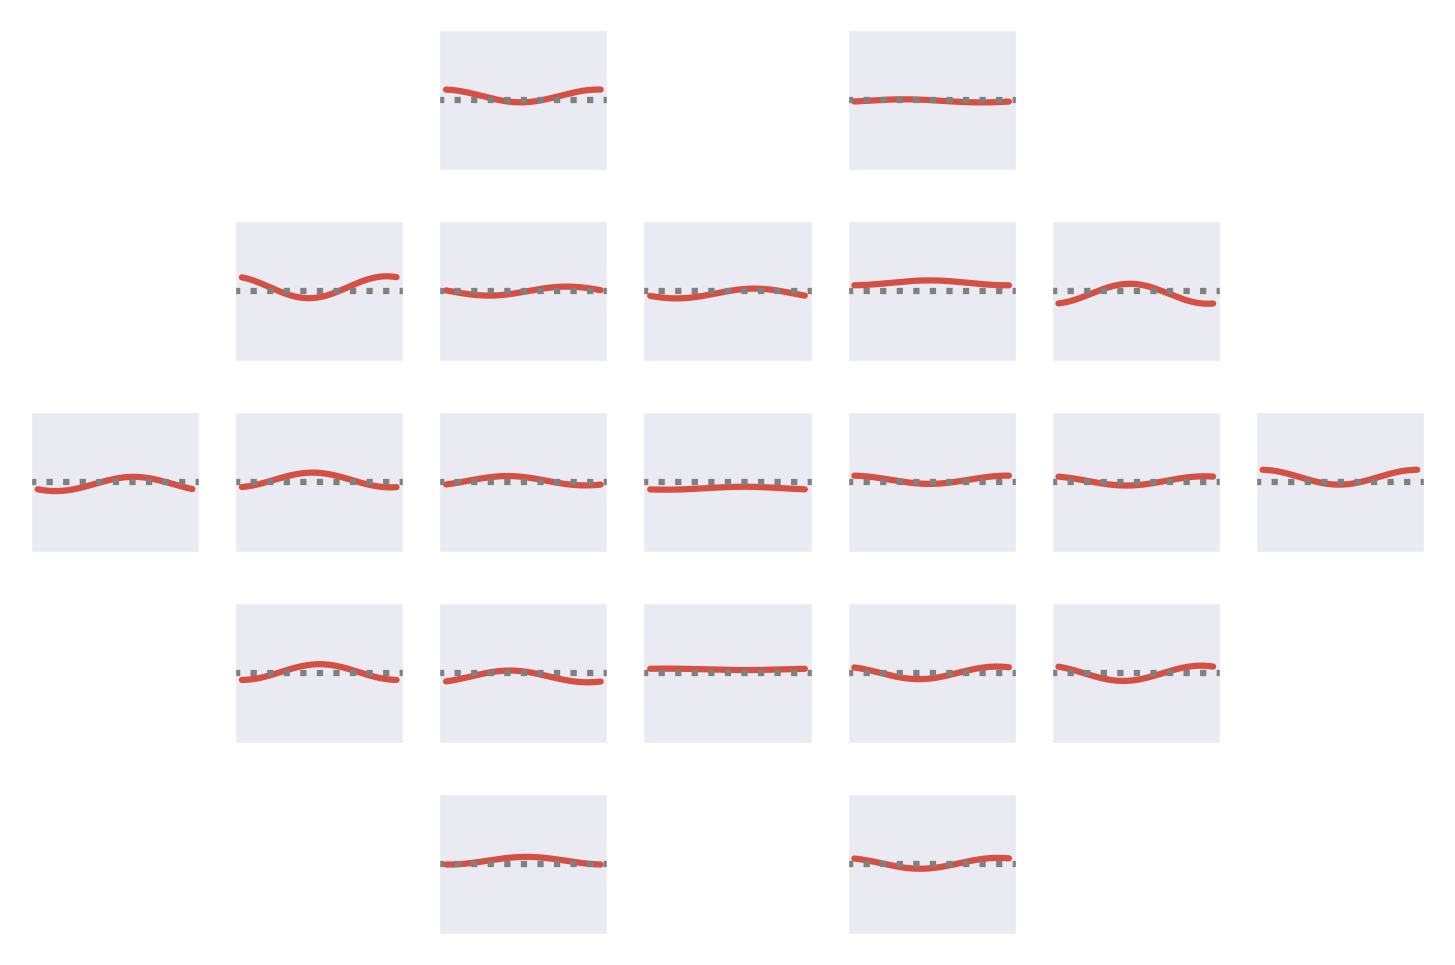
\includegraphics[width=.2\linewidth]{images/low-freq-prototypes-7.png}} \\
    
    \caption[Fourier-GMM means in input space]{
    \textbf{Means of the Fourier-GMM mixture components shown after
inversion into input space.} Note clearly visible frontal signals in the
components for the healthy class.
    }\label{low-freq-input-space-prototypes-fig}
\end{figure}



\begin{figure}[h!tb]
    \myfloatalign
    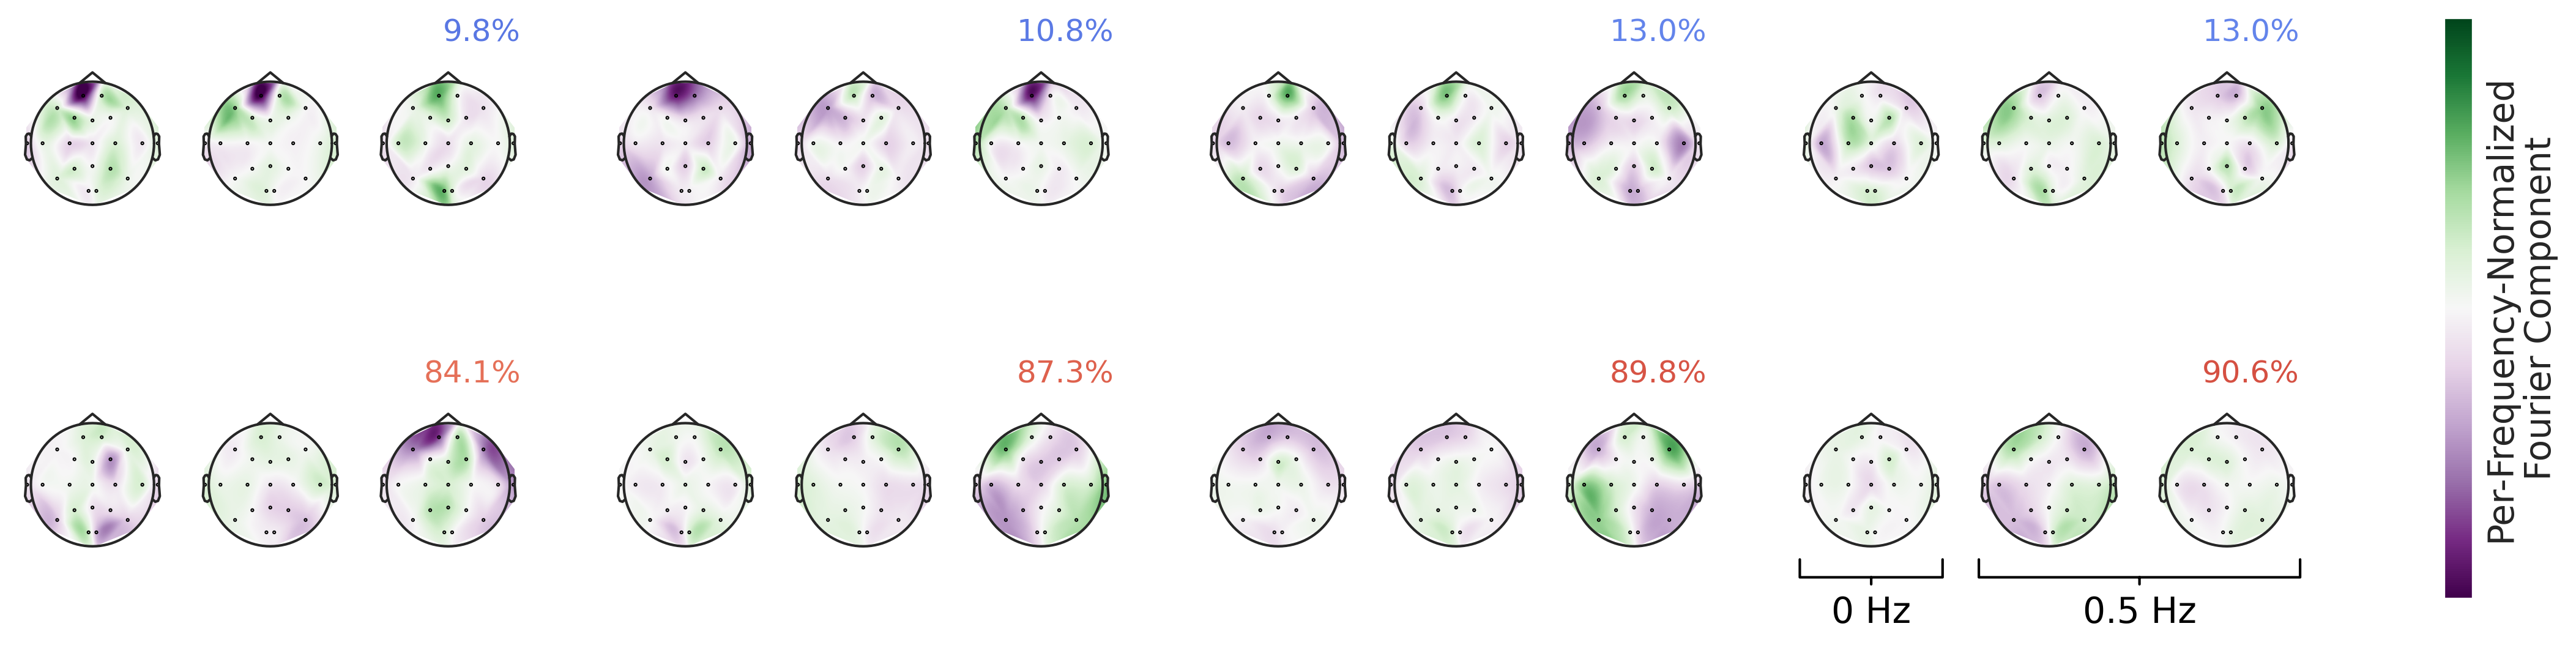
\includegraphics[width=1\linewidth]{images/low-freq-gmm-prototypes-scaled-per-freq-with-class-color-and-bar.png}
    \caption[Fourier-GMM means in Fourier space]{
\textbf{Means of the Fourier-GMM mixture components in Fourier space.}
Scalp plots for 0-Hz bin, real and imaginary values of 0.5-Hz bin.
Components sorted by pathological class weight, also shown as colored
text in top right of each component. Colormaps scaled per frequency bin.
Note strong frontal components for mixture components associated with
healthy class.
}
\label{fourier-gmm-low-freq-fig}
\end{figure}

Visualizations of the Fourier-GMM in
\Cref{low-freq-input-space-prototypes-fig} and \Cref{fourier-gmm-low-freq-fig} again show frontal
components associated with the healthy class and other components, with
spatial topographies that include temporal areas, associated with the
pathological class.

    Overall, the visualizations consistently indicate a frontal component
predictive for the healthy class and other components, with a spatial
topography that often includes temporal and nearby areas, predictive for
the pathological class.

\begin{openbox}
\item What other methods may help understand discriminative features in the EEG signal in the future?
\end{openbox}
